% =====================================================================
%  Chapter 7: Partial Derivatives, Differentials, and the Jacobian Matrix
%  Sections 7.1 and 7.2
% =====================================================================

\chapter{Partial Derivatives, Differentials, and the Jacobian Matrix}
\label{ch:7}

Chapter \ref{ch:6} gave us scalar fields, vector fields, level curves, level surfaces,
limits, and continuity.  We learned how to ask whether nearby inputs give nearby
outputs.

Now we ask a sharper question:

\[
    \text{How fast does the output change as the input moves?}
\]

For a single-variable function, there was only one input direction.  For a function
\[
    f(x,y),
\]
there are many.  A point can move east, north, northeast, or along a curved trail.  We
start with the simplest possible motions: move in one coordinate direction and freeze
the others.

\section{Partial derivatives}
\label{sec:7.1}

A contour map tells us where a function has the same value.  It does not tell us, by
itself, how fast the function changes when we step east or north.  To measure that,
we return to the single-variable derivative, but we use it on one slice at a time.

\subsection{Slicing a surface by holding variables fixed}

Picture a grassy hill behind an observatory.  Let \(x\) measure distance east and \(y\)
measure distance north, and suppose the height of the hill is modeled by
\[
    H(x,y)=80+3x-y-\frac14 x^2-\frac12 y^2.
\]
The height is measured in meters.  The input point \((x,y)\) is a point on the map.

At the point
\[
    P=(2,1),
\]
the height is
\[
    H(2,1)=80+6-1-1-\frac12=\frac{169}{2}=84.5.
\]

Now stand at \(P\) and walk directly east.  That means \(y\) stays fixed at \(1\), while
\(x\) changes.  Along this east-west slice, the height becomes the one-variable function
\[
    g(x)=H(x,1).
\]
Compute:
\[
\begin{aligned}
    g(x)
    &=
    80+3x-1-\frac14 x^2-\frac12        \\
    &=
    \frac{157}{2}+3x-\frac14 x^2.
\end{aligned}
\]
The slope of this slice at \(x=2\) is
\[
    g'(x)=3-\frac12 x,
\]
so
\[
    g'(2)=3-1=2.
\]
At \(P\), walking east raises the height at a rate of
\[
    2
\]
meters per unit of eastward distance.

Now stand at the same point and walk directly north.  This time \(x\) stays fixed at
\(2\), while \(y\) changes.  Along this north-south slice,
\[
    k(y)=H(2,y).
\]
Compute:
\[
\begin{aligned}
    k(y)
    &=
    80+6-y-1-\frac12y^2 \\
    &=
    85-y-\frac12y^2.
\end{aligned}
\]
Thus
\[
    k'(y)=-1-y,
\]
and
\[
    k'(1)=-2.
\]
At \(P\), walking north lowers the height at a rate of
\[
    2
\]
meters per unit of northward distance.

The same point has two different coordinate slopes:
\[
    \text{east slope}=2,
    \qquad
    \text{north slope}=-2.
\]

\begin{figure}[h]
\centering
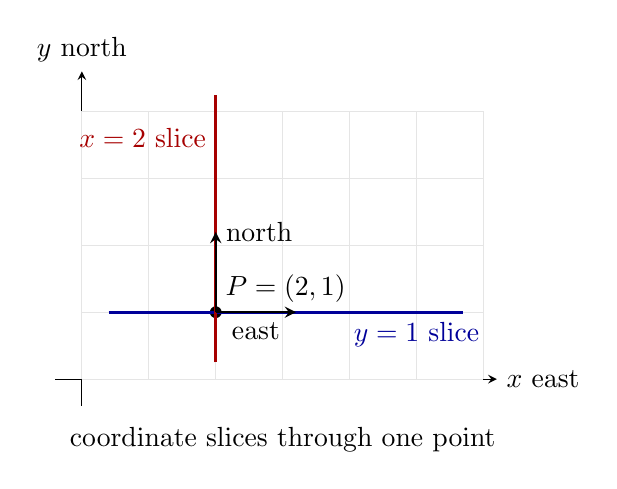
\begin{tikzpicture}[scale=0.85, >=stealth]
    \draw[->] (-0.4,0) -- (6.2,0) node[right] {\(x\) east};
    \draw[->] (0,-0.4) -- (0,4.6) node[above] {\(y\) north};

    \draw[gray!20, step=1] (0,0) grid (6,4);

    \fill (2,1) circle (2.5pt);
    \node[above right] at (2,1) {\(P=(2,1)\)};

    \draw[very thick, blue!60!black] (0.4,1) -- (5.7,1);
    \node[blue!60!black, below] at (5.0,1) {\(y=1\) slice};

    \draw[very thick, red!65!black] (2,0.25) -- (2,4.25);
    \node[red!65!black, left] at (2,3.6) {\(x=2\) slice};

    \draw[->, thick] (2,1) -- (3.2,1) node[midway, below] {east};
    \draw[->, thick] (2,1) -- (2,2.2) node[above, right] {north};

    \node at (3,-0.9) {coordinate slices through one point};
\end{tikzpicture}
\caption{To measure coordinate slopes, freeze one coordinate and let the other move.}
\end{figure}

This is the whole idea of a partial derivative.  We do not try to measure all possible
directions at once.  We take one coordinate direction and use the ordinary derivative
there.

\subsection{The meanings of \texorpdfstring{\(f_x\), \(f_y\), and \(f_z\)}{fx, fy, and fz}}

The east slope of \(H\) at \((2,1)\) came from differentiating with respect to \(x\),
while treating \(y\) as constant:
\[
    \frac{\partial H}{\partial x}(2,1)=2.
\]
The north slope came from differentiating with respect to \(y\), while treating \(x\)
as constant:
\[
    \frac{\partial H}{\partial y}(2,1)=-2.
\]

The symbol \(\partial\) reminds us that only part of the input is allowed to move.

\begin{definition}[Partial derivatives in two variables]
Let
\[
    f:D\subseteq\mathbb R^2\to\mathbb R.
\]
The partial derivative of \(f\) with respect to \(x\) at \((a,b)\) is
\[
\boxed{
    f_x(a,b)
    =
    \frac{\partial f}{\partial x}(a,b)
    =
    \lim_{h\to0}\frac{f(a+h,b)-f(a,b)}{h},
}
\]
when this limit exists.

The partial derivative of \(f\) with respect to \(y\) at \((a,b)\) is
\[
\boxed{
    f_y(a,b)
    =
    \frac{\partial f}{\partial y}(a,b)
    =
    \lim_{h\to0}\frac{f(a,b+h)-f(a,b)}{h},
}
\]
when this limit exists.
\end{definition}

These are ordinary derivatives hidden inside a two-variable function.

For the hill
\[
    H(x,y)=80+3x-y-\frac14 x^2-\frac12 y^2,
\]
we compute
\[
    H_x(x,y)=3-\frac12x,
\]
because \(y\) is treated as constant.  Also,
\[
    H_y(x,y)=-1-y,
\]
because \(x\) is treated as constant.

At \((2,1)\),
\[
    H_x(2,1)=2,
    \qquad
    H_y(2,1)=-2.
\]

\begin{example}[A canopy with two coordinate slopes]
A slanted fabric canopy over a market stall has height
\[
    C(x,y)=2+\frac{x}{4}+\frac{y}{6}.
\]
Then
\[
    C_x(x,y)=\frac14,
    \qquad
    C_y(x,y)=\frac16.
\]
So moving one meter east raises the canopy by \(\frac14\) meter, while moving one meter
north raises it by \(\frac16\) meter.

This canopy is a plane, so the coordinate slopes are the same at every point.
\end{example}

\begin{example}[A curved surface has slopes that change from point to point]
Let
\[
    B(x,y)=10-\frac{x^2}{4}-y^2.
\]
Then
\[
    B_x(x,y)=-\frac{x}{2},
    \qquad
    B_y(x,y)=-2y.
\]
At the top point \((0,0)\),
\[
    B_x(0,0)=0,
    \qquad
    B_y(0,0)=0.
\]
The surface is level in both coordinate directions.

At the point \((2,1)\),
\[
    B_x(2,1)=-1,
    \qquad
    B_y(2,1)=-2.
\]
There, the surface is descending eastward and descending more steeply northward.
\end{example}

\subsection{Units and interpretation in applications}

A partial derivative is a rate.  Its units tell the story.

Recall the bakery cost model from Chapter \ref{ch:6}:
\[
    C(u,v)=400+3u+4v+0.01uv,
\]
where \(u\) is the number of sourdough loaves and \(v\) is the number of rye loaves.
The output \(C(u,v)\) is measured in dollars.

Differentiate with respect to \(u\):
\[
    C_u(u,v)=3+0.01v.
\]
This means:

\[
    C_u(u,v)
    =
    \text{approximate extra cost per additional sourdough loaf,}
\]
while the number of rye loaves is held fixed.

Differentiate with respect to \(v\):
\[
    C_v(u,v)=4+0.01u.
\]
This means:

\[
    C_v(u,v)
    =
    \text{approximate extra cost per additional rye loaf,}
\]
while the number of sourdough loaves is held fixed.

At
\[
    (u,v)=(200,100),
\]
we get
\[
    C_u(200,100)=3+1=4,
\]
and
\[
    C_v(200,100)=4+2=6.
\]
Near that production level, one more sourdough loaf costs about \(4\) dollars, while
one more rye loaf costs about \(6\) dollars.

The phrase ``holding the other variable fixed'' is not decoration.  It is part of the
meaning of the derivative.

\subsection{Partial derivatives in three variables}

For a function of three variables,
\[
    f(x,y,z),
\]
there are three coordinate partial derivatives:
\[
    f_x,\qquad f_y,\qquad f_z.
\]
Each one measures the rate of change when one coordinate moves and the other two stay
fixed.

\begin{definition}[Partial derivatives in three variables]
Let
\[
    f:D\subseteq\mathbb R^3\to\mathbb R.
\]
At a point \((a,b,c)\),
\[
\boxed{
    f_x(a,b,c)
    =
    \lim_{h\to0}
    \frac{f(a+h,b,c)-f(a,b,c)}{h},
}
\]
\[
\boxed{
    f_y(a,b,c)
    =
    \lim_{h\to0}
    \frac{f(a,b+h,c)-f(a,b,c)}{h},
}
\]
and
\[
\boxed{
    f_z(a,b,c)
    =
    \lim_{h\to0}
    \frac{f(a,b,c+h)-f(a,b,c)}{h},
}
\]
when the limits exist.
\end{definition}

\begin{example}[Temperature in a storage room]
Let
\[
    T(x,y,z)=18+\frac{4}{1+x^2+y^2}-0.7z,
\]
where \(z\) is height above the floor in meters.  The last term says that higher shelves
are cooler.

The partial derivative with respect to \(z\) is
\[
    T_z(x,y,z)=-0.7.
\]
So, at every point, increasing height by one meter lowers the temperature by about
\(0.7^\circ\)C.

The \(x\)-partial derivative is
\[
    T_x(x,y,z)
    =
    -\frac{8x}{(1+x^2+y^2)^2}.
\]
The \(y\)-partial derivative is
\[
    T_y(x,y,z)
    =
    -\frac{8y}{(1+x^2+y^2)^2}.
\]
Those rates depend on where you are horizontally.
\end{example}

A vector-valued function can also have partial derivatives.  We differentiate each
component.

\begin{example}[Partial derivatives of a vector field]
The swirling field
\[
    \mathbf W(x,y)=(-y,x)
\]
has two components:
\[
    W_1(x,y)=-y,
    \qquad
    W_2(x,y)=x.
\]
So
\[
    \mathbf W_x(x,y)
    =
    \left(\frac{\partial}{\partial x}(-y),\frac{\partial}{\partial x}x\right)
    =
    (0,1),
\]
and
\[
    \mathbf W_y(x,y)
    =
    \left(\frac{\partial}{\partial y}(-y),\frac{\partial}{\partial y}x\right)
    =
    (-1,0).
\]
These vector partial derivatives tell us how the output arrow changes as the input
point moves east or north.

Later, in Section \ref{sec:7.5}, we will arrange these component derivatives into a
matrix.  That matrix is the Jacobian.
\end{example}

\subsection{A warning: coordinate slopes are not the whole surface}

It is tempting to believe that if the two coordinate slopes exist, then the function must
behave nicely near the point.  That is false.

Define
\[
    S(x,y)=
    \begin{cases}
    \dfrac{xy}{x^2+y^2}, & (x,y)\ne(0,0),\\[2mm]
    0, & (x,y)=(0,0).
    \end{cases}
\]
Compute the partial derivatives at the origin.

For the \(x\)-partial,
\[
    S_x(0,0)
    =
    \lim_{h\to0}\frac{S(h,0)-S(0,0)}{h}.
\]
But
\[
    S(h,0)=0
\]
for \(h\ne0\).  Therefore
\[
    S_x(0,0)=\lim_{h\to0}\frac{0-0}{h}=0.
\]

Similarly,
\[
    S_y(0,0)
    =
    \lim_{h\to0}\frac{S(0,h)-S(0,0)}{h}
    =
    0.
\]

So both partial derivatives exist at the origin, and both are \(0\).

But the function is not continuous at the origin.  Along the line \(y=x\),
\[
    S(x,x)=\frac{x^2}{2x^2}=\frac12
\]
for \(x\ne0\).  Along the \(x\)-axis,
\[
    S(x,0)=0.
\]
The two path limits disagree.

So the coordinate slices missed the problem.  The function looks flat along the two
axes, but it does not settle down near the origin.

This is the derivative version of the warning from Section \ref{sec:6.5}: checking only
coordinate directions does not check the whole plane.

Partial derivatives give the east and north slopes.  But a hiker is not limited to east
and north.  If the trail points northeast, the slope along the trail mixes the two
coordinate slopes.  The next question is how to measure the rate of change in a chosen
direction.

\section{Directional derivatives}
\label{sec:7.2}

Section \ref{sec:7.1} measured the change in a function when we moved along one
coordinate axis.  On a real hill, a trail almost never points exactly east or exactly north.
It points in some direction of its own.

A directional derivative measures the slope in that chosen direction.

\subsection{Rate of change in a chosen direction}

Return to the hill
\[
    H(x,y)=80+3x-y-\frac14x^2-\frac12y^2.
\]
At
\[
    P=(2,1),
\]
we found
\[
    H_x(2,1)=2,
    \qquad
    H_y(2,1)=-2.
\]
So east is uphill and north is downhill.

Now suppose a trail through \(P\) points in the direction
\[
    \mathbf u=\left(\frac35,\frac45\right).
\]
This is a unit vector because
\[
    \left(\frac35\right)^2+\left(\frac45\right)^2=1.
\]
Moving a signed distance \(t\) along the trail gives the point
\[
    (x(t),y(t))
    =
    (2,1)+t\left(\frac35,\frac45\right)
    =
    \left(2+\frac35t,\;1+\frac45t\right).
\]
The height along the trail is the one-variable function
\[
    g(t)=H\left(2+\frac35t,\;1+\frac45t\right).
\]
The slope of the hill along the trail at \(P\) is
\[
    g'(0).
\]

We can differentiate \(g(t)\) directly:
\[
\begin{aligned}
g(t)
&=
80
+3\left(2+\frac35t\right)
-\left(1+\frac45t\right) \\
&\qquad
-\frac14\left(2+\frac35t\right)^2
-\frac12\left(1+\frac45t\right)^2.
\end{aligned}
\]
Only the derivative at \(0\) is needed:
\[
\begin{aligned}
g'(0)
&=
3\left(\frac35\right)
-\frac45
-\frac12(2)\left(\frac35\right)
-(1)\left(\frac45\right)   \\
&=
\frac95-\frac45-\frac35-\frac45 \\
&=
-\frac25.
\end{aligned}
\]
So the trail slopes downward at
\[
    \frac25
\]
meter per unit distance.

\begin{figure}[h]
\centering
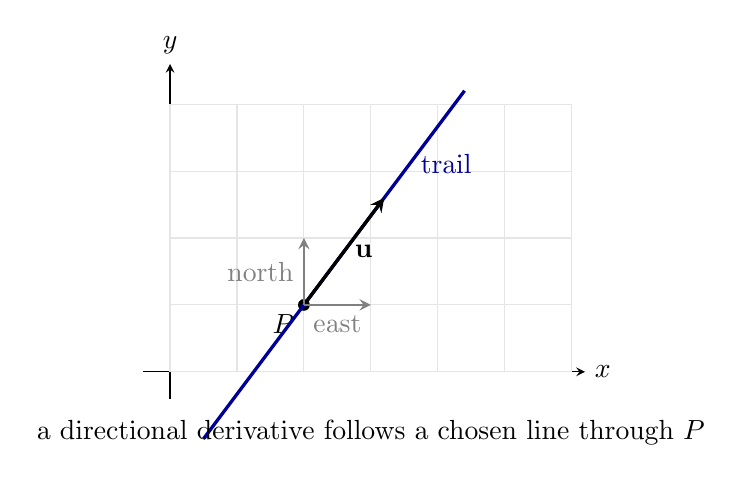
\begin{tikzpicture}[scale=0.85, >=stealth]
    \draw[->] (-0.4,0) -- (6.2,0) node[right] {\(x\)};
    \draw[->] (0,-0.4) -- (0,4.6) node[above] {\(y\)};

    \draw[gray!20, step=1] (0,0) grid (6,4);

    \fill (2,1) circle (2.5pt);
    \node[below left] at (2,1) {\(P\)};

    \draw[very thick, blue!60!black]
        (0.5,{1 + (4/3)*(0.5-2)}) -- (4.4,{1 + (4/3)*(4.4-2)});
    \node[blue!60!black, right] at (3.6,3.1) {trail};

    \draw[->, very thick] (2,1) -- ++(1.2,1.6)
        node[midway, right] {\(\mathbf u\)};

    \draw[->, thick, gray] (2,1) -- ++(1,0) node[midway, below] {east};
    \draw[->, thick, gray] (2,1) -- ++(0,1) node[midway, left] {north};

    \node at (3,-0.9) {a directional derivative follows a chosen line through \(P\)};
\end{tikzpicture}
\caption{A direction need not be a coordinate direction.}
\end{figure}

The calculation used only single-variable calculus after we turned the path into a
one-variable function.

\subsection{Directional derivatives from parametrized lines}

The same construction works for any scalar field.

Start at a point
\[
    \mathbf p=(a,b)
\]
and choose a unit direction
\[
    \mathbf u=(u_1,u_2).
\]
The line through \(\mathbf p\) in direction \(\mathbf u\) is
\[
    \mathbf r(t)=\mathbf p+t\mathbf u
    =
    (a+tu_1,b+tu_2).
\]
The function along the line is
\[
    g(t)=f(\mathbf r(t))=f(a+tu_1,b+tu_2).
\]
The directional derivative is \(g'(0)\).

\begin{definition}[Directional derivative]
Let
\[
    f:D\subseteq\mathbb R^2\to\mathbb R,
\]
let \(\mathbf p=(a,b)\), and let
\[
    \mathbf u=(u_1,u_2)
\]
be a unit vector.

The \emph{directional derivative of \(f\) at \(\mathbf p\) in the direction
\(\mathbf u\)} is
\[
\boxed{
    D_{\mathbf u}f(\mathbf p)
    =
    \lim_{t\to0}
    \frac{f(\mathbf p+t\mathbf u)-f(\mathbf p)}{t},
}
\]
when this limit exists.
\end{definition}

The same definition works in space.  If
\[
    \mathbf p=(a,b,c)
\]
and
\[
    \mathbf u=(u_1,u_2,u_3)
\]
is a unit vector, then
\[
\boxed{
    D_{\mathbf u}f(\mathbf p)
    =
    \lim_{t\to0}
    \frac{f(\mathbf p+t\mathbf u)-f(\mathbf p)}{t}.
}
\]

The vector \(\mathbf u\) is required to have length \(1\) so that \(t\) measures signed
distance along the line.  Otherwise the number would depend on how fast we chose to
walk through the same direction.

\begin{example}[Why the direction vector should be a unit vector]
Let
\[
    f(x,y)=x.
\]
At the origin, moving in the direction \((1,0)\) gives
\[
    \frac{f(t,0)-f(0,0)}{t}
    =
    \frac{t}{t}
    =
    1.
\]
So
\[
    D_{(1,0)}f(0,0)=1.
\]

If we tried to use the non-unit vector \((2,0)\), then the same line would be
parametrized by
\[
    (x,y)=(2t,0).
\]
The quotient would be
\[
    \frac{f(2t,0)-f(0,0)}{t}
    =
    \frac{2t}{t}
    =
    2.
\]
The direction did not change, but the answer doubled.  That is not a direction effect.
It is a speed effect.

Using unit vectors removes this ambiguity.
\end{example}

\subsection{The gradient formula for directional derivatives}

For the hill \(H\), the directional derivative along
\[
    \mathbf u=\left(\frac35,\frac45\right)
\]
was
\[
    -\frac25.
\]
There is a faster way to compute it.

At \(P=(2,1)\),
\[
    H_x(2,1)=2,
    \qquad
    H_y(2,1)=-2.
\]
Then
\[
\begin{aligned}
    H_x(2,1)\frac35+H_y(2,1)\frac45
    &=
    2\cdot\frac35+(-2)\cdot\frac45 \\
    &=
    \frac65-\frac85 \\
    &=
    -\frac25.
\end{aligned}
\]
This matches the direct calculation.

The two partial derivatives have combined with the two components of the direction
vector:
\[
    \left(H_x(2,1),H_y(2,1)\right)\cdot
    \left(\frac35,\frac45\right).
\]
The vector of partial derivatives has a name.

\begin{definition}[Gradient]
For a scalar-valued function
\[
    f(x,y),
\]
the \emph{gradient} of \(f\) is
\[
\boxed{
    \nabla f(x,y)=\left(f_x(x,y),f_y(x,y)\right).
}
\]

For a scalar-valued function
\[
    f(x,y,z),
\]
the gradient is
\[
\boxed{
    \nabla f(x,y,z)=\left(f_x(x,y,z),f_y(x,y,z),f_z(x,y,z)\right).
}
\]
\end{definition}

For the hill,
\[
    \nabla H(x,y)=\left(3-\frac12x,\,-1-y\right).
\]
At \((2,1)\),
\[
    \nabla H(2,1)=(2,-2).
\]
Thus
\[
    D_{\mathbf u}H(2,1)
    =
    \nabla H(2,1)\cdot\mathbf u.
\]

That formula is not an accident.  It works whenever the function is smooth enough near
the point.

\begin{theorem}[Gradient formula for directional derivatives]
Let
\[
    f:D\subseteq\mathbb R^2\to\mathbb R.
\]
Suppose \(f_x\) and \(f_y\) exist in a small disk around
\[
    \mathbf p=(a,b),
\]
and suppose \(f_x\) and \(f_y\) are continuous at \(\mathbf p\).

If \(\mathbf u=(u_1,u_2)\) is a unit vector, then
\[
\boxed{
    D_{\mathbf u}f(\mathbf p)
    =
    \nabla f(\mathbf p)\cdot\mathbf u.
}
\]
That is,
\[
\boxed{
    D_{\mathbf u}f(a,b)
    =
    f_x(a,b)u_1+f_y(a,b)u_2.
}
\]
\end{theorem}

\begin{proof}
Look at the change from
\[
    (a,b)
\]
to
\[
    (a+tu_1,b+tu_2).
\]
Split it into two coordinate changes:
\[
\begin{aligned}
&f(a+tu_1,b+tu_2)-f(a,b)\\
&\qquad =
\bigl[f(a+tu_1,b+tu_2)-f(a,b+tu_2)\bigr]
+
\bigl[f(a,b+tu_2)-f(a,b)\bigr].
\end{aligned}
\]
For the first bracket, only \(x\) changes.  By the one-variable Mean Value Theorem
applied to the \(x\)-slice, there is a number \(\theta_t\) between \(0\) and \(1\) such that
\[
    f(a+tu_1,b+tu_2)-f(a,b+tu_2)
    =
    tu_1\,f_x(a+\theta_ttu_1,b+tu_2).
\]
For the second bracket, only \(y\) changes.  Again by the one-variable Mean Value
Theorem, there is a number \(\eta_t\) between \(0\) and \(1\) such that
\[
    f(a,b+tu_2)-f(a,b)
    =
    tu_2\,f_y(a,b+\eta_ttu_2).
\]
Divide by \(t\):
\[
\begin{aligned}
\frac{f(a+tu_1,b+tu_2)-f(a,b)}{t}
&=
u_1\,f_x(a+\theta_ttu_1,b+tu_2)\\
&\qquad
+
u_2\,f_y(a,b+\eta_ttu_2).
\end{aligned}
\]
As \(t\to0\), the points inside \(f_x\) and \(f_y\) approach \((a,b)\).  Since the
partial derivatives are continuous at \((a,b)\),
\[
    f_x(a+\theta_ttu_1,b+tu_2)\to f_x(a,b),
\]
and
\[
    f_y(a,b+\eta_ttu_2)\to f_y(a,b).
\]
Therefore
\[
    D_{\mathbf u}f(a,b)=u_1f_x(a,b)+u_2f_y(a,b).
\]
\end{proof}

The same formula holds in space:
\[
\boxed{
    D_{\mathbf u}f(a,b,c)
    =
    \nabla f(a,b,c)\cdot\mathbf u,
}
\]
provided the first partial derivatives are continuous near the point.

\subsection{Why the continuity hypothesis is there}

The theorem required the partial derivatives to be continuous near the point.  Having
the two partial derivatives at the point is not enough.

Here is a function that shows what can go wrong:
\[
    f(x,y)=
    \begin{cases}
    \dfrac{x^2y}{x^2+y^2}, & (x,y)\ne(0,0),\\[2mm]
    0, & (x,y)=(0,0).
    \end{cases}
\]
First compute the partial derivatives at the origin.

Along the \(x\)-axis,
\[
    f(h,0)=0,
\]
so
\[
    f_x(0,0)
    =
    \lim_{h\to0}\frac{f(h,0)-f(0,0)}{h}
    =
    0.
\]
Along the \(y\)-axis,
\[
    f(0,h)=0,
\]
so
\[
    f_y(0,0)=0.
\]
Thus
\[
    \nabla f(0,0)=(0,0).
\]
If we tried to use the gradient formula without its hypotheses, it would predict
\[
    D_{\mathbf u}f(0,0)=0
\]
in every direction.

Now take the unit direction
\[
    \mathbf u=\left(\frac1{\sqrt2},\frac1{\sqrt2}\right).
\]
Then
\[
    t\mathbf u
    =
    \left(\frac{t}{\sqrt2},\frac{t}{\sqrt2}\right).
\]
For \(t\ne0\),
\[
\begin{aligned}
    f\left(\frac{t}{\sqrt2},\frac{t}{\sqrt2}\right)
    &=
    \frac{\left(\frac{t}{\sqrt2}\right)^2\left(\frac{t}{\sqrt2}\right)}
    {\left(\frac{t}{\sqrt2}\right)^2+\left(\frac{t}{\sqrt2}\right)^2} \\
    &=
    \frac{\frac{t^3}{2\sqrt2}}{t^2} \\
    &=
    \frac{t}{2\sqrt2}.
\end{aligned}
\]
Therefore
\[
\begin{aligned}
D_{\mathbf u}f(0,0)
&=
\lim_{t\to0}
\frac{f(t\mathbf u)-f(0,0)}{t} \\
&=
\lim_{t\to0}
\frac{\frac{t}{2\sqrt2}}{t} \\
&=
\frac1{2\sqrt2}.
\end{aligned}
\]
The directional derivative exists, but it is not \(0\).  The gradient formula fails.

The moral is precise:

\[
    \text{Partial derivatives at one point do not automatically combine into a true slope formula.}
\]

The continuity of the partial derivatives is one way to make sure the coordinate slices
fit together into one consistent local picture.  Section \ref{sec:7.3} will name that
picture: the total derivative.

\subsection{Fastest increase and steepest descent}

The gradient formula says
\[
    D_{\mathbf u}f(\mathbf p)=\nabla f(\mathbf p)\cdot\mathbf u.
\]
This turns a question about slopes into a question about the dot product.

For the hill at
\[
    P=(2,1),
\]
we found
\[
    \nabla H(2,1)=(2,-2).
\]
The gradient points east and south.  Its length is
\[
    \|\nabla H(2,1)\|
    =
    \sqrt{2^2+(-2)^2}
    =
    2\sqrt2.
\]
If we walk in the unit direction
\[
    \mathbf u=\frac{\nabla H(2,1)}{\|\nabla H(2,1)\|}
    =
    \left(\frac1{\sqrt2},-\frac1{\sqrt2}\right),
\]
then
\[
\begin{aligned}
D_{\mathbf u}H(2,1)
&=
\nabla H(2,1)\cdot\mathbf u\\
&=
\|\nabla H(2,1)\|\\
&=
2\sqrt2.
\end{aligned}
\]
That is the steepest uphill direction.

If we walk in the opposite direction,
\[
    -\mathbf u=
    \left(-\frac1{\sqrt2},\frac1{\sqrt2}\right),
\]
then
\[
    D_{-\mathbf u}H(2,1)=-2\sqrt2.
\]
That is the steepest downhill direction.

\begin{theorem}[Fastest increase and steepest descent]
Suppose the gradient formula holds at a point \(\mathbf p\), and suppose
\[
    \nabla f(\mathbf p)\ne\mathbf 0.
\]
Among all unit directions \(\mathbf u\),

\[
\boxed{
    D_{\mathbf u}f(\mathbf p)
}
\]
is largest when
\[
\boxed{
    \mathbf u=
    \frac{\nabla f(\mathbf p)}{\|\nabla f(\mathbf p)\|}.
}
\]
The largest value is
\[
\boxed{
    \|\nabla f(\mathbf p)\|.
}
\]

It is smallest when
\[
\boxed{
    \mathbf u=
    -\frac{\nabla f(\mathbf p)}{\|\nabla f(\mathbf p)\|}.
}
\]
The smallest value is
\[
\boxed{
    -\|\nabla f(\mathbf p)\|.
}
\]
\end{theorem}

\begin{proof}
For any unit vector \(\mathbf u\),
\[
    D_{\mathbf u}f(\mathbf p)
    =
    \nabla f(\mathbf p)\cdot\mathbf u.
\]
By the dot product formula,
\[
    \nabla f(\mathbf p)\cdot\mathbf u
    =
    \|\nabla f(\mathbf p)\|\,\|\mathbf u\|\cos\theta,
\]
where \(\theta\) is the angle between \(\nabla f(\mathbf p)\) and \(\mathbf u\).  Since
\[
    \|\mathbf u\|=1,
\]
this becomes
\[
    D_{\mathbf u}f(\mathbf p)
    =
    \|\nabla f(\mathbf p)\|\cos\theta.
\]
The largest possible value of \(\cos\theta\) is \(1\), when the two vectors point in the
same direction.  The smallest possible value is \(-1\), when they point in opposite
directions.
\end{proof}

If
\[
    \nabla f(\mathbf p)=\mathbf 0,
\]
then the gradient formula gives
\[
    D_{\mathbf u}f(\mathbf p)=0
\]
for every unit direction \(\mathbf u\).  In that case the first-order test sees no uphill or
downhill direction.  The point might be a peak, a valley, a saddle, or something flatter.
We will need second derivatives later to tell those apart.

\subsection{The gradient and contour maps}

The gradient also explains a feature of contour maps.

Suppose you walk along a level curve of \(f\).  The value of \(f\) stays constant, so the
rate of change along the curve is \(0\).  If \(\mathbf t\) is a unit tangent direction to the
level curve, then
\[
    D_{\mathbf t}f=\nabla f\cdot\mathbf t=0.
\]
So the gradient is perpendicular to the tangent direction of the level curve.

\[
    \text{The gradient points across contour lines, not along them.}
\]

\begin{figure}[h]
\centering
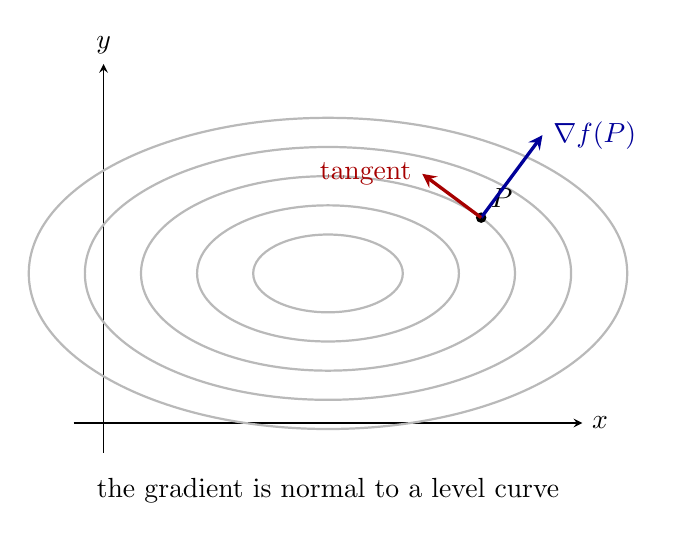
\begin{tikzpicture}[scale=0.95, >=stealth]
    \draw[->] (-0.4,0) -- (6.4,0) node[right] {\(x\)};
    \draw[->] (0,-0.4) -- (0,4.8) node[above] {\(y\)};

    % Draw contour ellipses
    \foreach \r in {0.8,1.4,2.0,2.6,3.2} {
        \draw[gray!55, thick] (3,2) ellipse ({1.25*\r} and {0.65*\r});
    }

    % P is on the r=2.0 ellipse at angle 35 degrees.
    % a = 1.25 * 2.0 = 2.5
    % b = 0.65 * 2.0 = 1.3
    \coordinate (P) at ({3 + 2.5*cos(35)}, {2 + 1.3*sin(35)});
    \fill (P) circle (2pt);
    \node[above right] at (P) {\(P\)};

    % True mathematical gradient (normal to the ellipse)
    % N = (cos(35)/a, sin(35)/b). Scaled by 2.5 for visual length.
    \draw[->, very thick, blue!60!black] (P) -- ++({2.5*cos(35)/2.5}, {2.5*sin(35)/1.3})
        node[right] {\(\nabla f(P)\)};

    % True mathematical tangent vector
    % T = (-a*sin(35), b*cos(35)). Scaled by 0.55 for visual length.
    \draw[->, very thick, red!65!black] (P) -- ++({-0.55*2.5*sin(35)}, {0.55*1.3*cos(35)})
        node[left] {tangent};

    \node at (3,-0.9) {the gradient is normal to a level curve};
\end{tikzpicture}
\caption{On a contour map, the gradient points in the direction of fastest increase,
perpendicular to the level curve.}
\end{figure}

This matches how hikers read contour maps.  Closely spaced contour lines mean steep
ground.  The steepest path crosses the contours as directly as possible.

The gradient packages the coordinate slopes into a vector.  Directional derivatives use
that vector to predict slopes along lines.  But the counterexample above left a gap: when
do the coordinate slopes really fit together into one reliable linear approximation?

That question leads to the main idea of multivariable differentiation.  Near a good point,
a curved surface should look like a plane, just as a curved graph in single-variable
calculus looked like a line.  The next section turns that sentence into a formula.
% Author note:
% The hill model used in Sections 7.1--7.2 has
% H(2,1)=167/2, not 169/2.  The calculations below use the corrected value.

\section{The total derivative as the best linear approximation}
\label{sec:7.3}

Section \ref{sec:7.2} measured slopes in chosen directions.  The gradient formula said
that, at a good point,
\[
    D_{\mathbf u}f(\mathbf p)=\nabla f(\mathbf p)\cdot \mathbf u.
\]
That formula is really a shadow of a larger idea.  Near a good point, the whole function
should be predicted by one linear rule.

\subsection{Why partial derivatives alone are not yet the derivative}

Return to the hill
\[
    H(x,y)=80+3x-y-\frac14x^2-\frac12y^2.
\]
At
\[
    P=(2,1),
\]
we found
\[
    H_x(2,1)=2,
    \qquad
    H_y(2,1)=-2.
\]
These two numbers tell us the east slope and the north slope.  But a small step on the
map may mix east and north.

Let the small displacement be
\[
    (\Delta x,\Delta y).
\]
Then the new point is
\[
    (2+\Delta x,\;1+\Delta y).
\]
Compute the height change:
\[
    H(2+\Delta x,1+\Delta y)-H(2,1).
\]
Since
\[
    H(2,1)=\frac{167}{2},
\]
we get
\[
\begin{aligned}
&H(2+\Delta x,1+\Delta y)-H(2,1)\\
&\qquad =
2\Delta x-2\Delta y
-\frac14(\Delta x)^2-\frac12(\Delta y)^2.
\end{aligned}
\]
The first part,
\[
    2\Delta x-2\Delta y,
\]
is linear in the displacement.  The remaining part,
\[
    -\frac14(\Delta x)^2-\frac12(\Delta y)^2,
\]
is quadratic.  For a small step, the quadratic terms are much smaller than the linear
terms.

For example, take
\[
    \Delta x=0.10,
    \qquad
    \Delta y=0.20.
\]
The linear prediction is
\[
    2(0.10)-2(0.20)=-0.20.
\]
The quadratic error is
\[
    -\frac14(0.10)^2-\frac12(0.20)^2
    =
    -0.0025-0.0200
    =
    -0.0225.
\]
So the actual height change is
\[
    -0.2225.
\]
The linear part predicted most of the change.  The error was smaller because it involved
squares of the step sizes.

This is what we want from a derivative in several variables.  It should not be only a
list of coordinate slopes.  It should be a linear machine that takes a small displacement
as input and returns the predicted change in the function.

For the hill at \(P\), that machine is
\[
    L(\Delta x,\Delta y)=2\Delta x-2\Delta y.
\]

\subsection{Linear approximation in two variables}

The same pattern appears for any well-behaved function \(f(x,y)\).  Near a point
\[
    (a,b),
\]
a small displacement
\[
    (\Delta x,\Delta y)
\]
should give
\[
    f(a+\Delta x,b+\Delta y)-f(a,b)
\]
approximately equal to a linear function of
\[
    (\Delta x,\Delta y).
\]
If the partial derivatives fit together correctly, that linear function is
\[
    f_x(a,b)\Delta x+f_y(a,b)\Delta y.
\]

So the local linear approximation is
\[
\boxed{
    f(a+\Delta x,b+\Delta y)
    \approx
    f(a,b)+f_x(a,b)\Delta x+f_y(a,b)\Delta y.
}
\]

Equivalently, if
\[
    x=a+\Delta x,
    \qquad
    y=b+\Delta y,
\]
then
\[
\boxed{
    f(x,y)
    \approx
    f(a,b)+f_x(a,b)(x-a)+f_y(a,b)(y-b).
}
\]

For the hill,
\[
    H(2+\Delta x,1+\Delta y)
    \approx
    H(2,1)+2\Delta x-2\Delta y.
\]
Since
\[
    H(2,1)=\frac{167}{2},
\]
this says
\[
    H(2+\Delta x,1+\Delta y)
    \approx
    \frac{167}{2}+2\Delta x-2\Delta y.
\]

The approximation is not merely a formula.  It is a plane pretending, for a short
distance, to be the curved surface.

\subsection{Differentiability and the total derivative}

The word \emph{differentiable} means that this linear prediction is genuinely the first
part of the change.

\begin{definition}[Differentiability in two variables]
Let
\[
    f:D\subseteq\mathbb R^2\to\mathbb R,
\]
and suppose
\[
    (a,b)
\]
is an interior point of \(D\).  We say that \(f\) is \emph{differentiable at \((a,b)\)} if
there is a linear function
\[
    L:\mathbb R^2\to\mathbb R
\]
such that
\[
\boxed{
    f(a+\Delta x,b+\Delta y)
    =
    f(a,b)+L(\Delta x,\Delta y)+R(\Delta x,\Delta y),
}
\]
where the error satisfies
\[
\boxed{
    \lim_{(\Delta x,\Delta y)\to(0,0)}
    \frac{|R(\Delta x,\Delta y)|}
    {\sqrt{(\Delta x)^2+(\Delta y)^2}}
    =
    0.
}
\]

The linear function \(L\) is called the \emph{total derivative} of \(f\) at \((a,b)\).  We
write
\[
    L=Df(a,b).
\]
\end{definition}

The error condition says more than
\[
    R(\Delta x,\Delta y)\to0.
\]
It says the error is small compared with the step length
\[
    \sqrt{(\Delta x)^2+(\Delta y)^2}.
\]
That is why the linear part is truly the first-order part of the change.

There is only one possible linear function \(L\).  If two linear functions both made the
error small in this sense, their difference would be a linear function that is smaller than
first order in every direction.  A nonzero linear function cannot do that.  Along any
direction where it is not zero, it grows exactly like the step length.

So it makes sense to say \emph{the} total derivative.

\begin{theorem}[The total derivative uses the partial derivatives]
If \(f\) is differentiable at \((a,b)\), then the partial derivatives
\[
    f_x(a,b),\qquad f_y(a,b)
\]
exist, and
\[
\boxed{
    Df(a,b)(\Delta x,\Delta y)
    =
    f_x(a,b)\Delta x+f_y(a,b)\Delta y.
}
\]
\end{theorem}

\begin{proof}
Because \(f\) is differentiable,
\[
    f(a+\Delta x,b+\Delta y)
    =
    f(a,b)+Df(a,b)(\Delta x,\Delta y)+R(\Delta x,\Delta y),
\]
where
\[
    \frac{|R(\Delta x,\Delta y)|}{\sqrt{(\Delta x)^2+(\Delta y)^2}}\to0.
\]

First move only in the \(x\)-direction.  Set
\[
    \Delta y=0.
\]
Then
\[
    f(a+\Delta x,b)-f(a,b)
    =
    Df(a,b)(\Delta x,0)+R(\Delta x,0).
\]
Divide by \(\Delta x\):
\[
    \frac{f(a+\Delta x,b)-f(a,b)}{\Delta x}
    =
    \frac{Df(a,b)(\Delta x,0)}{\Delta x}
    +
    \frac{R(\Delta x,0)}{\Delta x}.
\]
Since \(Df(a,b)\) is linear,
\[
    Df(a,b)(\Delta x,0)=\Delta x\,Df(a,b)(1,0).
\]
Also,
\[
    \frac{R(\Delta x,0)}{\Delta x}\to0.
\]
Therefore
\[
    f_x(a,b)=Df(a,b)(1,0).
\]

The same argument with
\[
    \Delta x=0
\]
gives
\[
    f_y(a,b)=Df(a,b)(0,1).
\]

Now use linearity.  Since
\[
    (\Delta x,\Delta y)=\Delta x(1,0)+\Delta y(0,1),
\]
we get
\[
\begin{aligned}
Df(a,b)(\Delta x,\Delta y)
&=
\Delta x\,Df(a,b)(1,0)+\Delta y\,Df(a,b)(0,1)\\
&=
f_x(a,b)\Delta x+f_y(a,b)\Delta y.
\end{aligned}
\]
\end{proof}

This theorem says that if the total derivative exists, then its formula is forced.  The
partial derivatives are the coefficients of the best linear approximation.

The converse is false.  Partial derivatives can exist without fitting together into a true
linear approximation.

\subsection{A warning: partial derivatives can fail to stitch together}

Section \ref{sec:7.2} gave the function
\[
    f(x,y)=
    \begin{cases}
    \dfrac{x^2y}{x^2+y^2}, & (x,y)\ne(0,0),\\[2mm]
    0, & (x,y)=(0,0).
    \end{cases}
\]
At the origin,
\[
    f_x(0,0)=0,
    \qquad
    f_y(0,0)=0.
\]
So if \(f\) were differentiable at the origin, the theorem would force
\[
    Df(0,0)(\Delta x,\Delta y)=0.
\]
The linear approximation would predict
\[
    f(\Delta x,\Delta y)\approx 0.
\]

But along the diagonal path
\[
    y=x,
\]
we have
\[
    f(x,x)=\frac{x^3}{2x^2}=\frac{x}{2}
\]
for \(x\ne0\).  The error, compared with the zero linear approximation, is
\[
    R(x,x)=\frac{x}{2}.
\]
The step length is
\[
    \sqrt{x^2+x^2}=\sqrt2\,|x|.
\]
Thus
\[
    \frac{|R(x,x)|}{\sqrt{x^2+x^2}}
    =
    \frac{|x|/2}{\sqrt2\,|x|}
    =
    \frac{1}{2\sqrt2}.
\]
This does not approach \(0\).

So \(f\) is not differentiable at the origin.

The partial derivatives at the origin saw only the two coordinate slices.  The total
derivative asks for one linear approximation that works for all small displacements at
once.  That is a stronger demand.

\subsection{Directional derivatives from the total derivative}

The total derivative explains why the gradient formula worked in Section
\ref{sec:7.2}.

Suppose \(f\) is differentiable at \(\mathbf p\), and let \(\mathbf u\) be a unit vector.
For small \(t\),
\[
    f(\mathbf p+t\mathbf u)
    =
    f(\mathbf p)+Df(\mathbf p)(t\mathbf u)+R(t\mathbf u).
\]
By linearity,
\[
    Df(\mathbf p)(t\mathbf u)=t\,Df(\mathbf p)(\mathbf u).
\]
So
\[
    \frac{f(\mathbf p+t\mathbf u)-f(\mathbf p)}{t}
    =
    Df(\mathbf p)(\mathbf u)+\frac{R(t\mathbf u)}{t}.
\]
The error term goes to \(0\), because
\[
    \frac{|R(t\mathbf u)|}{|t|}\to0.
\]
Therefore
\[
\boxed{
    D_{\mathbf u}f(\mathbf p)=Df(\mathbf p)(\mathbf u).
}
\]

In two variables,
\[
    Df(a,b)(u_1,u_2)
    =
    f_x(a,b)u_1+f_y(a,b)u_2,
\]
so
\[
\boxed{
    D_{\mathbf u}f(a,b)
    =
    \nabla f(a,b)\cdot\mathbf u.
}
\]

The gradient formula is therefore not the definition of differentiability.  It is a
consequence of differentiability.

\subsection{The tangent plane as a linear model}

For a function of one variable, differentiability means that the graph has a good tangent
line approximation:
\[
    f(a+\Delta x)\approx f(a)+f'(a)\Delta x.
\]
For a function of two variables, the graph is a surface, and the linear approximation is
a plane.

\begin{definition}[Tangent plane to a graph]
Suppose
\[
    z=f(x,y)
\]
and \(f\) is differentiable at \((a,b)\).  The tangent plane to the graph of \(f\) at
\[
    (a,b,f(a,b))
\]
is
\[
\boxed{
    z=
    f(a,b)+f_x(a,b)(x-a)+f_y(a,b)(y-b).
}
\]
\end{definition}

For the hill \(H\), at
\[
    (a,b)=(2,1),
\]
we have
\[
    H(2,1)=\frac{167}{2},
    \qquad
    H_x(2,1)=2,
    \qquad
    H_y(2,1)=-2.
\]
So the tangent plane is
\[
    z=\frac{167}{2}+2(x-2)-2(y-1).
\]
Simplifying,
\[
\boxed{
    z=\frac{163}{2}+2x-2y.
}
\]

\begin{figure}[h]
\centering
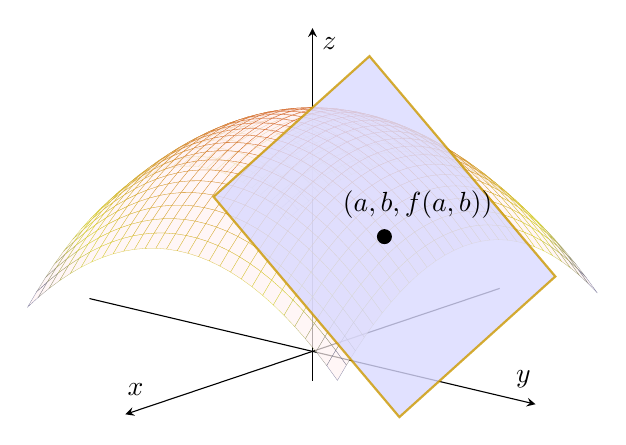
\begin{tikzpicture}
    \begin{axis}[
        view={130}{25},
        width=12cm, height=9cm,
        axis lines=center,
        xlabel={\(x\)}, ylabel={\(y\)}, zlabel={\(z\)},
        xmin=-3, xmax=3, ymin=-3, ymax=3, zmin=0, zmax=5,
        ticks=none,
        enlargelimits=0.1
    ]
        % The true curved surface
        \addplot3[
            surf,
            domain=-2.5:2.5,
            domain y=-2.5:2.5,
            samples=30,
            fill=red!5,
            draw=red!30!black,
            opacity=0.7,
            line width=0.1pt
        ] {4 - 0.25*(x^2 + y^2)};

        % The exact tangent plane at (1, 2, 2.75)
        \addplot3[
            surf,
            domain=-0.5:2.5,
            domain y=0.5:3.5,
            samples=2,
            fill=blue!15,
            draw=blue!60!black,
            thick,
            opacity=0.8
        ] {5.25 - 0.5*x - y};

        % The point of tangency
        \addplot3[
            mark=*,
            mark size=2.5pt,
            color=black
        ] coordinates {(1,2,2.75)};

        \node[above, xshift=1.2em, yshift=0.3em] 
            at (axis cs:1,2,2.75) {\((a,b,f(a,b))\)};

    \end{axis}
\end{tikzpicture}
\caption{A differentiable surface is locally modeled by its tangent plane.}
\end{figure}

The tangent plane does not claim that the surface is actually flat.  It says that, under a
magnifying glass centered at the point, the surface becomes harder and harder to
distinguish from this plane.

\subsection{Differentiability in \texorpdfstring{\(\mathbb R^n\)}{Rn}}

The definition does not depend on the plane.  It works in any number of input
variables.

\begin{definition}[Differentiability for scalar fields on \(\mathbb R^n\)]
Let
\[
    f:D\subseteq\mathbb R^n\to\mathbb R,
\]
and let \(\mathbf p\) be an interior point of \(D\).  We say that \(f\) is
\emph{differentiable at \(\mathbf p\)} if there is a linear function
\[
    L:\mathbb R^n\to\mathbb R
\]
such that
\[
\boxed{
    f(\mathbf p+\mathbf h)
    =
    f(\mathbf p)+L(\mathbf h)+R(\mathbf h),
}
\]
where
\[
\boxed{
    \lim_{\mathbf h\to\mathbf 0}
    \frac{|R(\mathbf h)|}{\|\mathbf h\|}=0.
}
\]
The linear function \(L\) is called the total derivative:
\[
    L=Df(\mathbf p).
\]
\end{definition}

If
\[
    \mathbf p=(a_1,\ldots,a_n),
\]
then differentiability forces
\[
\boxed{
    Df(\mathbf p)(h_1,\ldots,h_n)
    =
    f_{x_1}(\mathbf p)h_1+\cdots+f_{x_n}(\mathbf p)h_n.
}
\]

\begin{example}[A three-variable temperature model]
Recall the storage-room temperature model
\[
    T(x,y,z)=18+\frac{4}{1+x^2+y^2}-0.7z.
\]
At the point
\[
    (1,0,2),
\]
the temperature is
\[
    T(1,0,2)=18+\frac{4}{2}-1.4=18.6.
\]
The partial derivatives are
\[
    T_x(x,y,z)= -\frac{8x}{(1+x^2+y^2)^2},
\]
\[
    T_y(x,y,z)= -\frac{8y}{(1+x^2+y^2)^2},
\]
and
\[
    T_z(x,y,z)=-0.7.
\]
Thus
\[
    T_x(1,0,2)=-2,
    \qquad
    T_y(1,0,2)=0,
    \qquad
    T_z(1,0,2)=-0.7.
\]
The total derivative at \((1,0,2)\) is the linear function
\[
    DT(1,0,2)(\Delta x,\Delta y,\Delta z)
    =
    -2\Delta x-0.7\Delta z.
\]
A small move
\[
    (\Delta x,\Delta y,\Delta z)=(0.02,-0.03,0.10)
\]
therefore changes the temperature by about
\[
    -2(0.02)-0.7(0.10)
    =
    -0.11.
\]
So the model predicts a drop of about
\[
    0.11^\circ\text{C}.
\]
\end{example}

A three-variable scalar field has no ordinary graph in three-dimensional space, because
its graph would live in four dimensions:
\[
    (x,y,z,T(x,y,z)).
\]
But the total derivative still exists as a linear approximation.  The picture is no longer
a tangent plane we can draw.  The idea is the same: a nonlinear function is replaced,
near one point, by its best linear part.

The notation
\[
    Df(\mathbf p)(\mathbf h)
\]
is honest, but it is a little heavy.  The linear function \(Df(\mathbf p)\) eats a small
displacement \(\mathbf h\) and returns the predicted change in \(f\).  There is an older
notation that says the same thing in a way that will later become the language of line
integrals:
\[
    df=f_x\,dx+f_y\,dy.
\]
To make that formula more than a symbol, we have to decide what \(dx\) and \(dy\)
are.  We already met them as coordinate-reading linear functions.  Now they return
as the first examples of \(1\)-forms.

\section{Differentials}
\label{sec:7.4}

Section \ref{sec:7.3} made the total derivative into a linear function:
\[
    Df(\mathbf p)(\Delta\mathbf x).
\]
It takes a small displacement and returns the predicted change in \(f\).  Chapter
\ref{ch:3} already gave us the simplest linear functions:
\[
    dx,\qquad dy,\qquad dz.
\]
They read off components of a vector.  Differentials combine these component-readers
with the partial derivatives.

\subsection{The differential as a linear function of small changes}

Return to the bakery cost model from Section \ref{sec:7.1}:
\[
    C(u,v)=400+3u+4v+0.01uv,
\]
where \(u\) is the number of sourdough loaves and \(v\) is the number of rye loaves.

We computed
\[
    C_u(u,v)=3+0.01v,
    \qquad
    C_v(u,v)=4+0.01u.
\]
At
\[
    (u,v)=(200,100),
\]
these become
\[
    C_u(200,100)=4,
    \qquad
    C_v(200,100)=6.
\]
So the total derivative at this production level is
\[
    DC(200,100)(\Delta u,\Delta v)
    =
    4\Delta u+6\Delta v.
\]

Suppose the bakery changes production by
\[
    \Delta u=4,
    \qquad
    \Delta v=3.
\]
The linear prediction is
\[
    4(4)+6(3)=34.
\]
So the cost should increase by about \(34\) dollars.

The exact change is
\[
\begin{aligned}
&C(200+\Delta u,100+\Delta v)-C(200,100)\\
&\qquad =
4\Delta u+6\Delta v+0.01\Delta u\Delta v.
\end{aligned}
\]
For
\[
    \Delta u=4,\qquad \Delta v=3,
\]
this gives
\[
    34+0.01(4)(3)=34.12.
\]
The differential predicted the first-order part.  The extra
\[
    0.12
\]
came from the product of the two small changes.

\begin{definition}[Differential at a point]
If \(f\) is differentiable at \(\mathbf p\), then the \emph{differential of \(f\) at
\(\mathbf p\)} is the total derivative:
\[
\boxed{
    df_{\mathbf p}=Df(\mathbf p).
}
\]
Thus \(df_{\mathbf p}\) is a linear function of a small displacement.
\end{definition}

For the bakery,
\[
    dC_{(200,100)}(\Delta u,\Delta v)
    =
    4\Delta u+6\Delta v.
\]

The letter \(d\) is not decoration.  It means: take the first-order change.

\subsection{The notation \texorpdfstring{\(df=f_x\,dx+f_y\,dy\)}{df = fx dx + fy dy}}

The symbols
\[
    dx,\qquad dy
\]
are the coordinate-reading linear functions:
\[
    dx(\Delta x,\Delta y)=\Delta x,
\]
and
\[
    dy(\Delta x,\Delta y)=\Delta y.
\]
So if
\[
    f=f(x,y),
\]
then
\[
\begin{aligned}
df_{(a,b)}(\Delta x,\Delta y)
&=
f_x(a,b)\Delta x+f_y(a,b)\Delta y\\
&=
f_x(a,b)\,dx(\Delta x,\Delta y)
+
f_y(a,b)\,dy(\Delta x,\Delta y).
\end{aligned}
\]
This is why we write
\[
\boxed{
    df=f_x\,dx+f_y\,dy.
}
\]
At a specific point,
\[
\boxed{
    df_{(a,b)}
    =
    f_x(a,b)\,dx+f_y(a,b)\,dy.
}
\]

\begin{figure}[h]
\centering
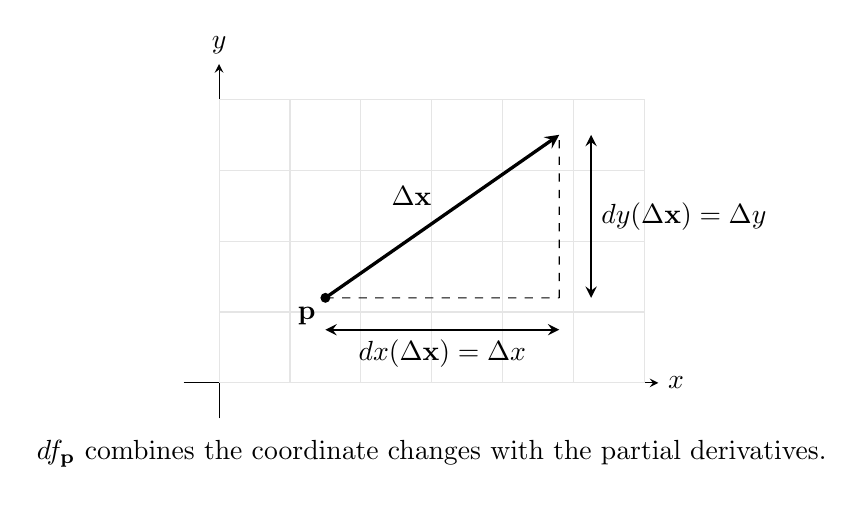
\begin{tikzpicture}[scale=0.9, >=stealth]
    \draw[->] (-0.5,0) -- (6.2,0) node[right] {\(x\)};
    \draw[->] (0,-0.5) -- (0,4.5) node[above] {\(y\)};

    \draw[gray!20, step=1] (0,0) grid (6,4);

    \coordinate (P) at (1.5,1.2);
    \coordinate (Q) at (4.8,3.5);

    \fill (P) circle (2pt);
    \node[below left] at (P) {\(\mathbf p\)};

    \draw[->, very thick] (P) -- (Q) node[midway, above left] {\(\Delta\mathbf x\)};

    \draw[dashed] (P) -- (4.8,1.2);
    \draw[dashed] (4.8,1.2) -- (Q);

    \draw[<->, thick] (1.5,0.75) -- (4.8,0.75)
        node[midway, below] {\(dx(\Delta\mathbf x)=\Delta x\)};

    \draw[<->, thick] (5.25,1.2) -- (5.25,3.5)
        node[midway, right] {\(dy(\Delta\mathbf x)=\Delta y\)};

    \node at (3,-1.0) {\(df_{\mathbf p}\) combines the coordinate changes with the partial derivatives.};
\end{tikzpicture}
\caption{The linear functions \(dx\) and \(dy\) read off the components of a displacement.}
\end{figure}

For functions of three variables,
\[
\boxed{
    df=f_x\,dx+f_y\,dy+f_z\,dz.
}
\]
At the point \((a,b,c)\),
\[
\boxed{
    df_{(a,b,c)}
    =
    f_x(a,b,c)\,dx+f_y(a,b,c)\,dy+f_z(a,b,c)\,dz.
}
\]

\begin{example}[The hill differential]
For
\[
    H(x,y)=80+3x-y-\frac14x^2-\frac12y^2,
\]
we have
\[
    H_x(x,y)=3-\frac12x,
    \qquad
    H_y(x,y)=-1-y.
\]
At
\[
    (2,1),
\]
\[
    H_x(2,1)=2,
    \qquad
    H_y(2,1)=-2.
\]
So
\[
\boxed{
    dH_{(2,1)}=2\,dx-2\,dy.
}
\]

If the trail direction is
\[
    \mathbf u=\left(\frac35,\frac45\right),
\]
then
\[
\begin{aligned}
dH_{(2,1)}(\mathbf u)
&=
2\,dx(\mathbf u)-2\,dy(\mathbf u)\\
&=
2\left(\frac35\right)-2\left(\frac45\right)\\
&=
-\frac25.
\end{aligned}
\]
This is exactly the directional derivative found in Section \ref{sec:7.2}.
\end{example}

The gradient and the differential contain the same coefficients, but they play different
roles:
\[
    \nabla f(a,b)=\bigl(f_x(a,b),f_y(a,b)\bigr)
\]
is a vector, while
\[
    df_{(a,b)}=f_x(a,b)\,dx+f_y(a,b)\,dy
\]
is a linear function that acts on displacement vectors.

The dot product connects them:
\[
    df_{\mathbf p}(\mathbf h)=\nabla f(\mathbf p)\cdot \mathbf h.
\]

\subsection{Error estimates and small-change calculations}

The differential is useful because it is the part of the change we can compute quickly.
If \(f\) is differentiable at \(\mathbf p\), then
\[
    f(\mathbf p+\Delta\mathbf x)-f(\mathbf p)
    =
    df_{\mathbf p}(\Delta\mathbf x)+R(\Delta\mathbf x),
\]
where
\[
    \frac{|R(\Delta\mathbf x)|}{\|\Delta\mathbf x\|}\to0.
\]
So for small changes,
\[
\boxed{
    \Delta f\approx df.
}
\]

This is the multivariable version of the single-variable estimate
\[
    \Delta y\approx f'(a)\Delta x.
\]

\begin{example}[Measuring the volume of a storage bin]
A rectangular storage bin has side lengths
\[
    x,\qquad y,\qquad z
\]
in meters.  Its volume is
\[
    V(x,y,z)=xyz.
\]
Then
\[
    V_x=yz,
    \qquad
    V_y=xz,
    \qquad
    V_z=xy.
\]
At
\[
    (x,y,z)=(2,3,5),
\]
we get
\[
    V_x=15,
    \qquad
    V_y=10,
    \qquad
    V_z=6.
\]
So
\[
    dV_{(2,3,5)}
    =
    15\,dx+10\,dy+6\,dz.
\]

Suppose the measured side lengths change by
\[
    dx=0.02,
    \qquad
    dy=-0.01,
    \qquad
    dz=0.03.
\]
Then
\[
\begin{aligned}
dV
&=
15(0.02)+10(-0.01)+6(0.03)\\
&=
0.30-0.10+0.18\\
&=
0.38.
\end{aligned}
\]
So the volume changes by about
\[
    0.38\ \text{m}^3.
\]

The exact change is
\[
    (2.02)(2.99)(5.03)-30
    =
    0.380194.
\]
The differential gives the first-order part.  The missing
\[
    0.000194
\]
comes from products of the small side-length changes.
\end{example}

Differentials are often used this way in measurements.  If the inputs have small errors,
the differential estimates the resulting output error.

\begin{example}[Temperature sensitivity]
For the storage-room temperature model
\[
    T(x,y,z)=18+\frac{4}{1+x^2+y^2}-0.7z,
\]
we found at \((1,0,2)\)
\[
    dT_{(1,0,2)}=-2\,dx-0.7\,dz.
\]
There is no \(dy\) term at that point because
\[
    T_y(1,0,2)=0.
\]
A small move
\[
    dx=0.02,\qquad dy=-0.03,\qquad dz=0.10
\]
therefore gives
\[
    dT=-2(0.02)-0.7(0.10)=-0.11.
\]
The \(dy\)-change does not affect the first-order estimate at this particular point.
\end{example}

A differential tells us which input errors matter most near the point.  The coefficient
of \(dx\) measures sensitivity to \(x\).  The coefficient of \(dy\) measures sensitivity to
\(y\).  The coefficient of \(dz\) measures sensitivity to \(z\).

\subsection{Differentials as the first examples of \texorpdfstring{\(1\)-forms}{1-forms}}

The expression
\[
    df=f_x\,dx+f_y\,dy
\]
is a special kind of object.  It is a rule that assigns, at each point, a linear function of
small displacements.

That is exactly the concrete meaning of a \(1\)-form.

\begin{definition}[\(1\)-form in the plane]
A \emph{\(1\)-form} on a region \(D\subseteq\mathbb R^2\) is an expression
\[
\boxed{
    \omega=P(x,y)\,dx+Q(x,y)\,dy.
}
\]
At a point
\[
    \mathbf p=(x,y),
\]
it acts on a displacement
\[
    \Delta\mathbf x=(\Delta x,\Delta y)
\]
by
\[
\boxed{
    \omega_{\mathbf p}(\Delta\mathbf x)
    =
    P(x,y)\Delta x+Q(x,y)\Delta y.
}
\]
\end{definition}

In space, a \(1\)-form has the form
\[
\boxed{
    \omega=P(x,y,z)\,dx+Q(x,y,z)\,dy+R(x,y,z)\,dz,
}
\]
and
\[
\boxed{
    \omega_{\mathbf p}(\Delta x,\Delta y,\Delta z)
    =
    P(\mathbf p)\Delta x+Q(\mathbf p)\Delta y+R(\mathbf p)\Delta z.
}
\]

A differential
\[
    df
\]
is a \(1\)-form:
\[
\boxed{
    df=f_x\,dx+f_y\,dy
}
\]
in the plane, and
\[
\boxed{
    df=f_x\,dx+f_y\,dy+f_z\,dz
}
\]
in space.

\begin{definition}[Exact \(1\)-form]
A \(1\)-form \(\omega\) is called \emph{exact} if there is a function \(f\) such that
\[
    \omega=df.
\]
\end{definition}

For example,
\[
    \omega=2x\,dx+2y\,dy
\]
is exact, because
\[
    \omega=d(x^2+y^2).
\]
But a general \(1\)-form need not come from a function.  The swirling form
\[
    \omega=-y\,dx+x\,dy
\]
is built from the vector field
\[
    \mathbf W(x,y)=(-y,x).
\]
At each point it measures how much a small displacement points with the swirl:
\[
    \omega_{(x,y)}(\Delta x,\Delta y)
    =
    -y\Delta x+x\Delta y.
\]
Whether such a form is a differential of some scalar field is a separate question.  We
will need line integrals and curl before we can answer it well.

For now, \(df\) is the bridge between ordinary functions and \(1\)-forms.  A function
has values.  Its differential measures first-order change.  A \(1\)-form is ready to be
added along a curve.

There is one more piece in this chapter before curves return.  A scalar function has one
differential:
\[
    df.
\]
A transformation
\[
    F=(F_1,F_2,\ldots,F_m)
\]
has one differential for each component:
\[
    dF_1,\quad dF_2,\quad \ldots,\quad dF_m.
\]
Stacking these linear functions into rows gives the matrix of the total derivative.  That
matrix is the Jacobian, and it tells how a nonlinear map moves small grids near a point.
\section{The Jacobian matrix}
\label{sec:7.5}

Section \ref{sec:7.4} turned the derivative of a scalar function into a \(1\)-form:
\[
    df=f_x\,dx+f_y\,dy.
\]
That was one linear function.  But many transformations have several output
components.  Each component has its own differential, and those differentials want to
be stacked.

That stack is the Jacobian matrix.

\subsection{A rubber sheet map}

Imagine a square grid printed on a thin rubber sheet.  The sheet is pulled so that a
point \((x,y)\) moves to a new point
\[
    F(x,y)=(X(x,y),Y(x,y)).
\]
Suppose the rule is
\[
\boxed{
    F(x,y)=
    \left(
        x+\frac15xy,\;
        y+\frac1{10}x^2
    \right).
}
\]
This is not a linear transformation, because of the terms \(xy\) and \(x^2\).  But near
one point it should look almost linear if the point is viewed closely enough.

Take
\[
    P=(2,1).
\]
Then
\[
    F(2,1)=
    \left(
        2+\frac25,\;
        1+\frac4{10}
    \right)
    =
    \left(\frac{12}{5},\frac75\right).
\]

Now make a small step
\[
    (\Delta x,\Delta y)
\]
from \(P\).  The new point is
\[
    (2+\Delta x,\;1+\Delta y).
\]
Compute the change in the first output:
\[
\begin{aligned}
X(2+\Delta x,1+\Delta y)-X(2,1)
&=
\left(2+\Delta x+\frac15(2+\Delta x)(1+\Delta y)\right)-\frac{12}{5}\\
&=
\frac65\Delta x+\frac25\Delta y+\frac15\Delta x\,\Delta y.
\end{aligned}
\]
The linear part is
\[
    \frac65\Delta x+\frac25\Delta y.
\]

Now compute the change in the second output:
\[
\begin{aligned}
Y(2+\Delta x,1+\Delta y)-Y(2,1)
&=
\left(1+\Delta y+\frac1{10}(2+\Delta x)^2\right)-\frac75\\
&=
\frac25\Delta x+\Delta y+\frac1{10}(\Delta x)^2.
\end{aligned}
\]
The linear part is
\[
    \frac25\Delta x+\Delta y.
\]

So near \(P\),
\[
\boxed{
    F(2+\Delta x,1+\Delta y)
    \approx
    F(2,1)
    +
    \left(
        \frac65\Delta x+\frac25\Delta y,\;
        \frac25\Delta x+\Delta y
    \right).
}
\]
The linear machine acting on the small displacement is
\[
    (\Delta x,\Delta y)
    \longmapsto
    \left(
        \frac65\Delta x+\frac25\Delta y,\;
        \frac25\Delta x+\Delta y
    \right).
\]
As a matrix, this is
\[
\boxed{
    \begin{pmatrix}
        \frac65 & \frac25\\[1mm]
        \frac25 & 1
    \end{pmatrix}
    \begin{pmatrix}
        \Delta x\\
        \Delta y
    \end{pmatrix}.
}
\]

That matrix is the derivative of the transformation \(F\) at \(P\).

\begin{figure}[h]
\centering
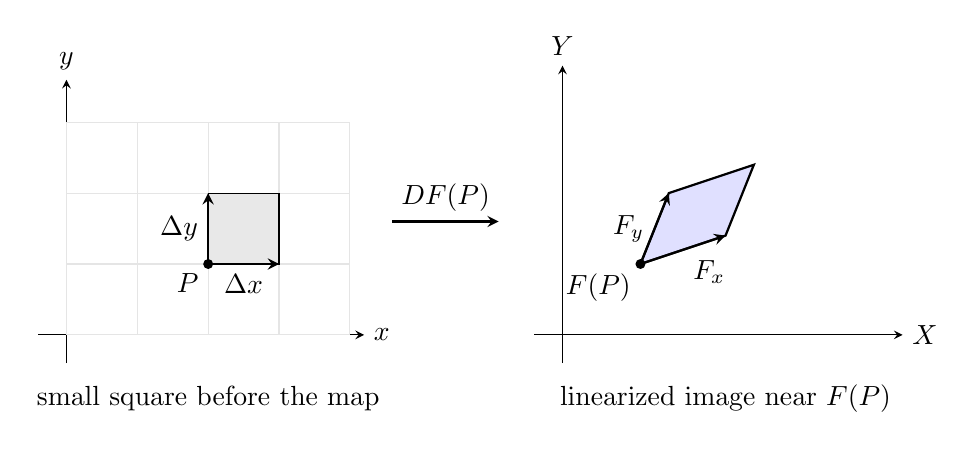
\begin{tikzpicture}[scale=0.9, >=stealth]
    \begin{scope}
        \draw[->] (-0.4,0) -- (4.2,0) node[right] {\(x\)};
        \draw[->] (0,-0.4) -- (0,3.6) node[above] {\(y\)};
        \draw[gray!20, step=1] (0,0) grid (4,3);

        \coordinate (P) at (2,1);
        \draw[fill=gray!18] (2,1) -- (3,1) -- (3,2) -- (2,2) -- cycle;
        \fill (P) circle (2pt);
        \node[below left] at (P) {\(P\)};

        \draw[->, thick] (2,1) -- (3,1) node[midway, below] {\(\Delta x\)};
        \draw[->, thick] (2,1) -- (2,2) node[midway, left] {\(\Delta y\)};

        \node at (2,-0.9) {small square before the map};
    \end{scope}

    \begin{scope}[shift={(7,0)}]
        \draw[->] (-0.4,0) -- (4.8,0) node[right] {\(X\)};
        \draw[->] (0,-0.4) -- (0,3.8) node[above] {\(Y\)};

        \coordinate (Q) at (1.1,1.0);
        \coordinate (A) at (2.3,1.4);
        \coordinate (B) at (1.5,2.0);
        \coordinate (AB) at (2.7,2.4);

        \draw[fill=blue!12, thick] (Q) -- (A) -- (AB) -- (B) -- cycle;
        \fill (Q) circle (2pt);
        \node[below left] at (Q) {\(F(P)\)};

        \draw[->, thick] (Q) -- (A) node[midway, below right] {\(F_x\)};
        \draw[->, thick] (Q) -- (B) node[midway, left] {\(F_y\)};

        \node at (2.3,-0.9) {linearized image near \(F(P)\)};
    \end{scope}

    \draw[->, thick] (4.6,1.6) -- (6.1,1.6) node[midway, above] {\(DF(P)\)};
\end{tikzpicture}
\caption{Near one point, a nonlinear map sends a small square almost to a
parallelogram.  The derivative matrix gives that parallelogram.}
\end{figure}

\subsection{Derivatives of transformations}

A scalar function has one output.  A transformation
\[
    F:\mathbb R^n\to\mathbb R^m
\]
has \(m\) output components:
\[
    F(\mathbf x)=
    \bigl(F_1(\mathbf x),F_2(\mathbf x),\ldots,F_m(\mathbf x)\bigr).
\]
Each component \(F_i\) is a scalar-valued function.

The derivative should be the best linear map from input displacements to output
displacements.

\begin{definition}[Differentiability of a transformation]
Let
\[
    F:D\subseteq\mathbb R^n\to\mathbb R^m,
\]
and let \(\mathbf p\) be an interior point of \(D\).  We say that \(F\) is
\emph{differentiable at \(\mathbf p\)} if there is a linear map
\[
    A:\mathbb R^n\to\mathbb R^m
\]
such that
\[
\boxed{
    F(\mathbf p+\mathbf h)
    =
    F(\mathbf p)+A\mathbf h+\mathbf R(\mathbf h),
}
\]
where
\[
\boxed{
    \lim_{\mathbf h\to\mathbf 0}
    \frac{\|\mathbf R(\mathbf h)\|}{\|\mathbf h\|}=0.
}
\]
The linear map \(A\) is called the \emph{total derivative} of \(F\) at \(\mathbf p\), and
we write
\[
    A=DF(\mathbf p).
\]
\end{definition}

This is the vector-valued version of the definition in Section \ref{sec:7.3}.  The only
change is that the error is now a vector, so we measure its size with a norm.

If
\[
    F=(F_1,\ldots,F_m)
\]
is differentiable at \(\mathbf p\), then each component \(F_i\) is differentiable at
\(\mathbf p\).  Its differential gives one row of the derivative matrix.

\subsection{The Jacobian matrix}

Let
\[
    F:\mathbb R^n\to\mathbb R^m
\]
have component functions
\[
    F_1,\ldots,F_m.
\]
Use input coordinates
\[
    x_1,x_2,\ldots,x_n.
\]
The partial derivatives form an \(m\times n\) matrix:
\[
\boxed{
J_F(\mathbf p)
=
\begin{pmatrix}
\dfrac{\partial F_1}{\partial x_1}(\mathbf p)
&
\dfrac{\partial F_1}{\partial x_2}(\mathbf p)
&
\cdots
&
\dfrac{\partial F_1}{\partial x_n}(\mathbf p)
\\[3mm]
\dfrac{\partial F_2}{\partial x_1}(\mathbf p)
&
\dfrac{\partial F_2}{\partial x_2}(\mathbf p)
&
\cdots
&
\dfrac{\partial F_2}{\partial x_n}(\mathbf p)
\\
\vdots & \vdots & \ddots & \vdots
\\[1mm]
\dfrac{\partial F_m}{\partial x_1}(\mathbf p)
&
\dfrac{\partial F_m}{\partial x_2}(\mathbf p)
&
\cdots
&
\dfrac{\partial F_m}{\partial x_n}(\mathbf p)
\end{pmatrix}.
}
\]
This matrix is called the \emph{Jacobian matrix} of \(F\) at \(\mathbf p\).  It is also
called the \emph{Jacobi matrix}.

When \(F\) is differentiable at \(\mathbf p\), the Jacobian matrix is the matrix of the
linear map \(DF(\mathbf p)\):
\[
\boxed{
    DF(\mathbf p)(\mathbf h)=J_F(\mathbf p)\mathbf h.
}
\]

For the rubber sheet map,
\[
    F(x,y)=
    \left(
        x+\frac15xy,\;
        y+\frac1{10}x^2
    \right),
\]
we have
\[
    F_1(x,y)=x+\frac15xy,
    \qquad
    F_2(x,y)=y+\frac1{10}x^2.
\]
The partial derivatives are
\[
    \frac{\partial F_1}{\partial x}=1+\frac15y,
    \qquad
    \frac{\partial F_1}{\partial y}=\frac15x,
\]
and
\[
    \frac{\partial F_2}{\partial x}=\frac15x,
    \qquad
    \frac{\partial F_2}{\partial y}=1.
\]
So
\[
\boxed{
    J_F(x,y)
    =
    \begin{pmatrix}
        1+\frac15y & \frac15x\\[1mm]
        \frac15x & 1
    \end{pmatrix}.
}
\]
At \(P=(2,1)\),
\[
\boxed{
    J_F(2,1)
    =
    \begin{pmatrix}
        \frac65 & \frac25\\[1mm]
        \frac25 & 1
    \end{pmatrix}.
}
\]
This is exactly the matrix found by expanding the map near \(P\).

\subsection{Rows as differentials of component functions}

The row viewpoint is the one that connects directly to differentials.

For
\[
    F=(F_1,F_2),
\]
the component differentials are
\[
    dF_1=F_{1x}\,dx+F_{1y}\,dy,
\]
and
\[
    dF_2=F_{2x}\,dx+F_{2y}\,dy.
\]
At a point \(P\), these become
\[
    dF_{1,P}=F_{1x}(P)\,dx+F_{1y}(P)\,dy,
\]
\[
    dF_{2,P}=F_{2x}(P)\,dx+F_{2y}(P)\,dy.
\]
Stacking them gives
\[
\boxed{
    J_F(P)
    =
    \begin{pmatrix}
        \text{coefficients of }dF_{1,P}\\
        \text{coefficients of }dF_{2,P}
    \end{pmatrix}.
}
\]

For the rubber sheet map at \(P=(2,1)\),
\[
    dF_{1,P}=\frac65\,dx+\frac25\,dy,
\]
and
\[
    dF_{2,P}=\frac25\,dx+dy.
\]
Therefore
\[
    J_F(P)
    =
    \begin{pmatrix}
        \frac65 & \frac25\\[1mm]
        \frac25 & 1
    \end{pmatrix}.
\]

Rows measure how each output coordinate changes.

Columns tell a different story.  The first column is the output change caused by a tiny
step in the \(x\)-direction:
\[
    F_x(P)=
    \begin{pmatrix}
        F_{1x}(P)\\
        F_{2x}(P)
    \end{pmatrix}.
\]
The second column is the output change caused by a tiny step in the \(y\)-direction:
\[
    F_y(P)=
    \begin{pmatrix}
        F_{1y}(P)\\
        F_{2y}(P)
    \end{pmatrix}.
\]
So the rows are differentials of component functions, while the columns are images of
coordinate directions.

Both views are useful.

\subsection{Local linearization of nonlinear maps}

The Jacobian matrix gives the linear approximation:
\[
\boxed{
    F(\mathbf p+\mathbf h)
    \approx
    F(\mathbf p)+J_F(\mathbf p)\mathbf h.
}
\]
In coordinates, for a map
\[
    F(x,y)=(F_1(x,y),F_2(x,y)),
\]
near \((a,b)\),
\[
\boxed{
\begin{aligned}
F_1(a+\Delta x,b+\Delta y)
&\approx
F_1(a,b)
+
F_{1x}(a,b)\Delta x
+
F_{1y}(a,b)\Delta y,\\
F_2(a+\Delta x,b+\Delta y)
&\approx
F_2(a,b)
+
F_{2x}(a,b)\Delta x
+
F_{2y}(a,b)\Delta y.
\end{aligned}
}
\]
This is just the scalar linear approximation applied to each component.

\begin{example}[A small displacement through the rubber map]
Use
\[
    F(x,y)=
    \left(
        x+\frac15xy,\;
        y+\frac1{10}x^2
    \right)
\]
at
\[
    P=(2,1),
\]
and take
\[
    \mathbf h=(0.03,-0.04).
\]
The linear prediction is
\[
\begin{aligned}
J_F(P)\mathbf h
&=
\begin{pmatrix}
\frac65 & \frac25\\[1mm]
\frac25 & 1
\end{pmatrix}
\begin{pmatrix}
0.03\\
-0.04
\end{pmatrix}  \\
&=
\begin{pmatrix}
\frac65(0.03)+\frac25(-0.04)\\[1mm]
\frac25(0.03)-0.04
\end{pmatrix}  \\
&=
\begin{pmatrix}
0.020\\
-0.028
\end{pmatrix}.
\end{aligned}
\]
So
\[
    F(2.03,0.96)
    \approx
    F(2,1)+(0.020,-0.028).
\]
Since
\[
    F(2,1)=\left(\frac{12}{5},\frac75\right)=(2.4,1.4),
\]
the prediction is
\[
    F(2.03,0.96)\approx(2.420,1.372).
\]

The exact value is
\[
\begin{aligned}
F(2.03,0.96)
&=
\left(
2.03+\frac15(2.03)(0.96),\;
0.96+\frac1{10}(2.03)^2
\right)\\
&=
(2.41976,\;1.37209).
\end{aligned}
\]
The Jacobian gave the first-order change.  The remaining error came from products and
squares of the small displacement components.
\end{example}

\subsection{A parametrized surface and its Jacobian}

The Jacobian matrix also works when the output dimension is larger than the input
dimension.

Let
\[
    \mathbf s(u,v)=
    \left(
        u,\;
        v,\;
        2+\frac{u^2}{4}-\frac{v^2}{9}
    \right).
\]
This is a parametrized surface:
\[
    \mathbf s:\mathbb R^2\to\mathbb R^3.
\]
The component functions are
\[
    s_1(u,v)=u,
    \qquad
    s_2(u,v)=v,
    \qquad
    s_3(u,v)=2+\frac{u^2}{4}-\frac{v^2}{9}.
\]
The Jacobian matrix is
\[
\boxed{
J_{\mathbf s}(u,v)
=
\begin{pmatrix}
1 & 0\\
0 & 1\\[1mm]
\frac{u}{2} & -\frac{2v}{9}
\end{pmatrix}.
}
\]
This is a \(3\times2\) matrix.  It cannot have a determinant, because it is not square.

Its columns are
\[
    \mathbf s_u(u,v)=
    \left(1,0,\frac{u}{2}\right),
\]
and
\[
    \mathbf s_v(u,v)=
    \left(0,1,-\frac{2v}{9}\right).
\]
These are tangent directions on the surface.  A tiny step in the \(u\)-direction becomes
\(\mathbf s_u\).  A tiny step in the \(v\)-direction becomes \(\mathbf s_v\).

At
\[
    (u,v)=(2,3),
\]
the tangent directions are
\[
    \mathbf s_u(2,3)=(1,0,1),
\]
and
\[
    \mathbf s_v(2,3)=\left(0,1,-\frac23\right).
\]
So near the surface point
\[
    \mathbf s(2,3)=
    \left(2,3,2+1-1\right)=(2,3,2),
\]
the surface is locally approximated by
\[
\boxed{
    \mathbf s(2+\Delta u,3+\Delta v)
    \approx
    (2,3,2)
    +
    \Delta u(1,0,1)
    +
    \Delta v\left(0,1,-\frac23\right).
}
\]
This is a tangent plane written in vector form.

\subsection{The Jacobian determinant as local area or volume scaling}

A determinant appears only when the Jacobian matrix is square:
\[
    F:\mathbb R^n\to\mathbb R^n.
\]
Then
\[
    \det J_F(\mathbf p)
\]
measures signed local scaling.

For a map
\[
    F(x,y)=(X(x,y),Y(x,y)),
\]
the Jacobian determinant is
\[
\boxed{
    \frac{\partial(X,Y)}{\partial(x,y)}
    =
    \det
    \begin{pmatrix}
        X_x & X_y\\
        Y_x & Y_y
    \end{pmatrix}
    =
    X_xY_y-X_yY_x.
}
\]
At a point, this number tells how a tiny signed area is scaled.

For the rubber sheet map,
\[
    J_F(2,1)
    =
    \begin{pmatrix}
        \frac65 & \frac25\\[1mm]
        \frac25 & 1
    \end{pmatrix}.
\]
Therefore
\[
\boxed{
    \det J_F(2,1)
    =
    \frac65\cdot1-\frac25\cdot\frac25
    =
    \frac{26}{25}.
}
\]
So a very small area near \(P=(2,1)\) is expanded by a factor of about
\[
    \frac{26}{25}=1.04.
\]
The determinant is positive, so the local orientation is preserved.

The same fact can be written in the language of \(2\)-forms.  Since
\[
    dX=X_x\,dx+X_y\,dy
\]
and
\[
    dY=Y_x\,dx+Y_y\,dy,
\]
we get
\[
\begin{aligned}
dX\wedge dY
&=
(X_x\,dx+X_y\,dy)\wedge(Y_x\,dx+Y_y\,dy)\\
&=
X_xY_y\,dx\wedge dy+X_yY_x\,dy\wedge dx\\
&=
(X_xY_y-X_yY_x)\,dx\wedge dy.
\end{aligned}
\]
Thus
\[
\boxed{
    dX\wedge dY
    =
    \det(J_F)\,dx\wedge dy.
}
\]
The determinant is the coefficient that converts the old signed area form into the new
signed area form.

In three variables, if
\[
    F(x,y,z)=(X,Y,Z),
\]
then
\[
\boxed{
    dX\wedge dY\wedge dZ
    =
    \det(J_F)\,dx\wedge dy\wedge dz.
}
\]
Now the determinant measures signed local volume scaling.

This is why the Jacobian determinant will appear in change of variables for double and
triple integrals.  A coordinate change does not merely rename points.  It stretches tiny
areas and volumes, and the determinant measures that stretching.

The Jacobian matrix is a promise: near a point, the transformation behaves like this
linear map.  But the promise is only true when the partial derivatives really stitch
together into a total derivative.  The next question is practical and sharp: when can we
trust the matrix of partial derivatives to be the derivative?

\section{Sufficient conditions and warning examples}
\label{sec:7.6}

The Jacobian matrix in Section \ref{sec:7.5} was built from partial derivatives.  That is
natural, but it hides a danger.  Partial derivatives are measured along coordinate slices.
The total derivative must work for every small displacement at once.

So we need a test that says when the slices fit together.

\subsection{A safe example first}

Return to the rubber sheet map
\[
    F(x,y)=
    \left(
        x+\frac15xy,\;
        y+\frac1{10}x^2
    \right).
\]
Its partial derivatives are
\[
    F_{1x}=1+\frac15y,
    \qquad
    F_{1y}=\frac15x,
\]
and
\[
    F_{2x}=\frac15x,
    \qquad
    F_{2y}=1.
\]
These are polynomial functions.  They are continuous everywhere.

That means the entries of the Jacobian matrix do not jump or oscillate near the point.
A nearby point has nearby coordinate slopes.  The local grid is not being asked to
change its linear behavior abruptly at microscopic scale.

This is the good situation.  In it, the Jacobian matrix is the total derivative.

\begin{theorem}[Continuous partial derivatives imply differentiability]
Let
\[
    f:D\subseteq\mathbb R^2\to\mathbb R,
\]
and let \((a,b)\) be an interior point of \(D\).  Suppose \(f_x\) and \(f_y\) exist in a
small disk around \((a,b)\), and suppose both partial derivatives are continuous at
\((a,b)\).  Then \(f\) is differentiable at \((a,b)\), and
\[
\boxed{
    Df(a,b)(\Delta x,\Delta y)
    =
    f_x(a,b)\Delta x+f_y(a,b)\Delta y.
}
\]
\end{theorem}

\begin{proof}
We compare
\[
    f(a+\Delta x,b+\Delta y)
\]
to
\[
    f(a,b).
\]
Split the change into two coordinate moves:
\[
\begin{aligned}
&f(a+\Delta x,b+\Delta y)-f(a,b)\\
&\qquad =
\bigl[f(a+\Delta x,b+\Delta y)-f(a,b+\Delta y)\bigr]
+
\bigl[f(a,b+\Delta y)-f(a,b)\bigr].
\end{aligned}
\]
For the first bracket, only \(x\) changes.  By the one-variable Mean Value Theorem,
there is a number \(\theta\) between \(0\) and \(1\) such that
\[
    f(a+\Delta x,b+\Delta y)-f(a,b+\Delta y)
    =
    \Delta x\,
    f_x(a+\theta\Delta x,b+\Delta y).
\]
For the second bracket, only \(y\) changes.  There is a number \(\eta\) between
\(0\) and \(1\) such that
\[
    f(a,b+\Delta y)-f(a,b)
    =
    \Delta y\,
    f_y(a,b+\eta\Delta y).
\]
Subtract the proposed linear part:
\[
    f_x(a,b)\Delta x+f_y(a,b)\Delta y.
\]
The error is
\[
\begin{aligned}
R(\Delta x,\Delta y)
&=
\Delta x\bigl[
f_x(a+\theta\Delta x,b+\Delta y)-f_x(a,b)
\bigr]\\
&\qquad
+
\Delta y\bigl[
f_y(a,b+\eta\Delta y)-f_y(a,b)
\bigr].
\end{aligned}
\]
Let
\[
    r=\sqrt{(\Delta x)^2+(\Delta y)^2}.
\]
Since
\[
    |\Delta x|\le r,
    \qquad
    |\Delta y|\le r,
\]
we get
\[
\begin{aligned}
\frac{|R(\Delta x,\Delta y)|}{r}
&\le
\left|
f_x(a+\theta\Delta x,b+\Delta y)-f_x(a,b)
\right|\\
&\qquad+
\left|
f_y(a,b+\eta\Delta y)-f_y(a,b)
\right|.
\end{aligned}
\]
As
\[
    (\Delta x,\Delta y)\to(0,0),
\]
the points inside \(f_x\) and \(f_y\) approach \((a,b)\).  Since \(f_x\) and \(f_y\)
are continuous at \((a,b)\), the right side approaches \(0\).  Therefore
\[
    \frac{|R(\Delta x,\Delta y)|}{r}\to0,
\]
which is exactly differentiability.
\end{proof}

The same test works in any finite number of variables and for vector-valued maps.

\begin{theorem}[Jacobian test for differentiability]
Let
\[
    F:D\subseteq\mathbb R^n\to\mathbb R^m
\]
have component functions
\[
    F_1,\ldots,F_m.
\]
Suppose all first partial derivatives
\[
    \frac{\partial F_i}{\partial x_j}
\]
exist in a small ball around \(\mathbf p\), and suppose all of them are continuous at
\(\mathbf p\).  Then \(F\) is differentiable at \(\mathbf p\), and
\[
\boxed{
    DF(\mathbf p)(\mathbf h)=J_F(\mathbf p)\mathbf h.
}
\]
\end{theorem}

The proof is just the scalar theorem applied to each component.  The component
errors are each smaller than first order, so the vector error is also smaller than first
order.

This theorem is one of the most useful tests in the course.  For polynomials,
trigonometric functions, exponentials, logarithms on their domains, and rational
functions away from zero denominators, the partial derivatives are continuous.  In those
settings, the Jacobian matrix really is the derivative.

Now come the warnings.

\subsection{Continuous partials are sufficient, not necessary}

The theorem gives a reliable test.  It is not an if-and-only-if statement.  A function can
be differentiable even when its partial derivatives are not continuous.

Define
\[
    f(x,y)=
    \begin{cases}
    x^2\sin\left(\dfrac1x\right), & x\ne0,\\[2mm]
    0, & x=0.
    \end{cases}
\]
This function does not depend on \(y\).  At the origin,
\[
    f_x(0,0)
    =
    \lim_{h\to0}
    \frac{h^2\sin(1/h)-0}{h}
    =
    \lim_{h\to0}h\sin(1/h)
    =
    0,
\]
and
\[
    f_y(0,0)=0.
\]
So the candidate total derivative at the origin is the zero linear function.

To check differentiability, estimate the error:
\[
    |f(x,y)|
    =
    \left|x^2\sin\left(\frac1x\right)\right|
    \le x^2
\]
when \(x\ne0\), and the same inequality is true when \(x=0\).  Since
\[
    x^2\le x^2+y^2,
\]
we get
\[
    \frac{|f(x,y)-0|}{\sqrt{x^2+y^2}}
    \le
    \sqrt{x^2+y^2}
    \to0.
\]
Therefore \(f\) is differentiable at the origin.

But \(f_x\) is not continuous at the origin.  For \(x\ne0\),
\[
    f_x(x,y)=
    2x\sin\left(\frac1x\right)
    -
    \cos\left(\frac1x\right).
\]
The term
\[
    \cos\left(\frac1x\right)
\]
oscillates as \(x\to0\).  So \(f_x(x,y)\) does not approach \(f_x(0,0)=0\).

The moral is one-way:

\[
    \text{continuous partial derivatives guarantee differentiability,}
\]
but
\[
    \text{differentiability does not require continuous partial derivatives.}
\]

The theorem is a safe test, not the only possible route.

\subsection{Partial derivatives can exist without continuity}

A sharper warning comes from the function
\[
    S(x,y)=
    \begin{cases}
    \dfrac{xy}{x^2+y^2}, & (x,y)\ne(0,0),\\[2mm]
    0, & (x,y)=(0,0).
    \end{cases}
\]
We met this kind of example when studying limits.  Along the \(x\)-axis,
\[
    S(x,0)=0.
\]
Along the \(y\)-axis,
\[
    S(0,y)=0.
\]
Therefore
\[
    S_x(0,0)=0,
    \qquad
    S_y(0,0)=0.
\]
Both partial derivatives exist at the origin.

But \(S\) is not continuous at the origin.  Along the diagonal \(y=x\),
\[
    S(x,x)=\frac{x^2}{2x^2}=\frac12
\]
for \(x\ne0\).  Along the \(x\)-axis,
\[
    S(x,0)=0.
\]
The function does not settle down to one value near the origin.

Since differentiability always implies continuity, \(S\) cannot be differentiable at the
origin.

So partial derivatives at a point do not even guarantee continuity.  They only check
two coordinate slices.

\subsection{Partial derivatives can exist without differentiability}

The previous example failed because the function was not continuous.  The next one is
more subtle: the function is continuous, and the partial derivatives exist, but the total
derivative still fails.

Define
\[
    G(x,y)=
    \begin{cases}
    \dfrac{x^2y}{x^2+y^2}, & (x,y)\ne(0,0),\\[2mm]
    0, & (x,y)=(0,0).
    \end{cases}
\]
First, \(G\) is continuous at the origin.  For \((x,y)\ne(0,0)\),
\[
    |G(x,y)|
    =
    \frac{|x|^2|y|}{x^2+y^2}
    \le
    |y|.
\]
Since
\[
    |y|\le \sqrt{x^2+y^2},
\]
we get
\[
    |G(x,y)|\to0
\]
as \((x,y)\to(0,0)\).  Thus
\[
    G(x,y)\to G(0,0).
\]

Now compute the partial derivatives at the origin.  Along the \(x\)-axis,
\[
    G(h,0)=0,
\]
so
\[
    G_x(0,0)=
    \lim_{h\to0}\frac{G(h,0)-G(0,0)}{h}
    =
    0.
\]
Along the \(y\)-axis,
\[
    G(0,h)=0,
\]
so
\[
    G_y(0,0)=0.
\]
If \(G\) were differentiable at the origin, its total derivative would have to be
\[
    DG(0,0)(\Delta x,\Delta y)=0.
\]
The tangent plane formula would predict
\[
    z=0.
\]

Now test the diagonal path
\[
    y=x.
\]
For \(x\ne0\),
\[
    G(x,x)=
    \frac{x^3}{2x^2}
    =
    \frac{x}{2}.
\]
The proposed linear approximation is \(0\), so the error along this path is
\[
    R(x,x)=\frac{x}{2}.
\]
The input step length is
\[
    \sqrt{x^2+x^2}=\sqrt2\,|x|.
\]
Therefore
\[
    \frac{|R(x,x)|}{\sqrt{x^2+x^2}}
    =
    \frac{|x|/2}{\sqrt2\,|x|}
    =
    \frac1{2\sqrt2}.
\]
This does not approach \(0\).

So \(G\) is not differentiable at the origin.

The function is continuous.  The two coordinate partial derivatives exist.  But no
linear approximation works in all small directions at once.

\subsection{The tangent plane formula can fail without differentiability}

The graph of \(G\) gives the geometric warning.

Since
\[
    G_x(0,0)=0,
    \qquad
    G_y(0,0)=0,
\]
the formal tangent plane formula would give
\[
    z=0.
\]
Along the coordinate axes, that plane looks correct:
\[
    G(x,0)=0,
    \qquad
    G(0,y)=0.
\]
But along the diagonal,
\[
    G(x,x)=\frac{x}{2}.
\]
The graph rises with a nonzero first-order slope along a direction that the coordinate
slices missed.

A tangent plane is not a plane that matches two coordinate traces.  It is a plane that
matches the whole surface to first order.  That is why differentiability is the real
condition behind the tangent plane.

For \((x,y)\ne(0,0)\), the partial derivatives of \(G\) are
\[
    G_x(x,y)=\frac{2xy^3}{(x^2+y^2)^2},
\]
and
\[
    G_y(x,y)=\frac{x^2(x^2-y^2)}{(x^2+y^2)^2}.
\]
These partial derivatives are not continuous at the origin.  For example, along
\(y=x\),
\[
    G_x(x,x)=\frac12,
\]
while
\[
    G_x(0,0)=0.
\]
So the continuous-partials theorem did not apply, and the failure was real.

\subsection{What the test gives us}

For most functions built from familiar smooth pieces, the Jacobian matrix can be trusted.
For example,
\[
    F(x,y,z)=
    \left(
        e^{xy}+z,\;
        \sin(xz)+y^2
    \right)
\]
has continuous partial derivatives everywhere.  So \(F\) is differentiable everywhere,
and
\[
    DF(x,y,z)(\Delta x,\Delta y,\Delta z)
    =
    J_F(x,y,z)
    \begin{pmatrix}
        \Delta x\\
        \Delta y\\
        \Delta z
    \end{pmatrix}.
\]
The Jacobian is
\[
\boxed{
J_F(x,y,z)
=
\begin{pmatrix}
    ye^{xy} & xe^{xy} & 1\\
    z\cos(xz) & 2y & x\cos(xz)
\end{pmatrix}.
}
\]
This is a \(2\times3\) matrix because the input has three coordinates and the output
has two.

Near any point, this matrix gives the first-order response of the two outputs to a small
movement in space.

The chapter has now turned derivatives into linear maps.  That viewpoint changes how
the chain rule looks.  If a moving particle passes through a temperature field, or if one
coordinate change follows another, the nonlinear functions should first be replaced by
their local linear parts.  Linear parts compose by matrix multiplication.  That is the
next return of the single-variable chain rule, now written in the language of Jacobian
matrices.
\section{Chapter review and applications}
\label{sec:7.7}

This chapter began with coordinate slopes and ended with a matrix.  The path was
shorter than it may have looked:
\[
    \text{small change}
    \quad\longrightarrow\quad
    \text{linear prediction}
    \quad\longrightarrow\quad
    \text{matrix of that prediction}.
\]
The derivative in several variables is not a number.  It is the best linear rule for
predicting what a function does to a small displacement.

\subsection*{A map of the chapter}

\[
\begin{array}{c|p{8.8cm}}
\text{Idea} & \text{What it means} \\ \hline
f_x(a,b)
&
The rate of change when \(x\) moves and \(y\) is held fixed.\\[1mm]

f_y(a,b)
&
The rate of change when \(y\) moves and \(x\) is held fixed.\\[1mm]

D_{\mathbf u}f(\mathbf p)
&
The rate of change at \(\mathbf p\) in the unit direction \(\mathbf u\).\\[1mm]

\nabla f(\mathbf p)
&
The vector of partial derivatives.  When the function is differentiable,
\[
    D_{\mathbf u}f(\mathbf p)=\nabla f(\mathbf p)\cdot\mathbf u.
\]
\\[3mm]

Df(\mathbf p)
&
The total derivative: the linear function that gives the first-order change in
\(f\) near \(\mathbf p\).\\[1mm]

df_{\mathbf p}
&
Another name for \(Df(\mathbf p)\).  Written as
\[
    df_{\mathbf p}=f_x(\mathbf p)\,dx+f_y(\mathbf p)\,dy
\]
in two variables.\\[3mm]

\text{\(1\)-form}
&
A rule such as
\[
    P\,dx+Q\,dy
\]
that eats a small displacement and returns a number.  A differential \(df\) is the
first example.\\[3mm]

\text{tangent plane}
&
The graph of the linear approximation:
\[
    z=f(a,b)+f_x(a,b)(x-a)+f_y(a,b)(y-b).
\]
\\[3mm]

J_F(\mathbf p)
&
The Jacobian matrix of a transformation \(F\).  Its rows are the differentials of the
component functions.\\[1mm]

\det J_F(\mathbf p)
&
For a map \(\mathbb R^n\to\mathbb R^n\), the signed local area or volume scaling
factor.
\end{array}
\]

The safest practical test was this:

\[
\boxed{
\text{If the first partial derivatives are continuous near the point, then the function
is differentiable there.}
}
\]

The warning was just as important:

\[
\boxed{
\text{Partial derivatives at one point do not guarantee differentiability.}
}
\]

Coordinate slices can lie.  The total derivative asks for one linear approximation that
works in every small direction at once.

\subsection*{One model, four readings}

A vineyard has a thin protective canopy over a rectangular patch of young plants.  The
height of the canopy above the ground is modeled by
\[
    A(x,y)
    =
    6+\frac25x-\frac15y-\frac{3}{100}x^2-\frac1{50}y^2,
\]
where \(x\) and \(y\) are measured in meters, and \(A\) is measured in meters.

At the point
\[
    P=(3,2),
\]
the height is
\[
\begin{aligned}
    A(3,2)
    &=
    6+\frac65-\frac25-\frac{27}{100}-\frac4{50}  \\
    &=
    \frac{129}{20}.
\end{aligned}
\]

First compute the partial derivatives:
\[
    A_x(x,y)=\frac25-\frac{3}{50}x,
\]
and
\[
    A_y(x,y)=-\frac15-\frac1{25}y.
\]
At \(P\),
\[
    A_x(3,2)=\frac{11}{50},
    \qquad
    A_y(3,2)=-\frac7{25}.
\]

So a small eastward step raises the canopy at about
\[
    \frac{11}{50}
\]
meter per meter, while a small northward step lowers it at about
\[
    \frac7{25}
\]
meter per meter.

The gradient is
\[
    \nabla A(3,2)=\left(\frac{11}{50},-\frac7{25}\right).
\]

The differential is the linear function
\[
\boxed{
    dA_{(3,2)}=
    \frac{11}{50}\,dx-\frac7{25}\,dy.
}
\]
If a worker moves by
\[
    \Delta x=0.20,
    \qquad
    \Delta y=-0.10,
\]
then the first-order height change is
\[
\begin{aligned}
    dA_{(3,2)}(0.20,-0.10)
    &=
    \frac{11}{50}(0.20)-\frac7{25}(-0.10)\\
    &=
    0.044+0.028\\
    &=
    0.072.
\end{aligned}
\]
The exact height change is
\[
    0.072-\frac{3}{100}(0.20)^2-\frac1{50}(-0.10)^2
    =
    0.0706.
\]
The differential predicted the first-order part.  The missing
\[
    -0.0014
\]
came from the quadratic terms.

Now take the unit direction
\[
    \mathbf u=\left(\frac35,\frac45\right).
\]
The directional derivative at \(P\) is
\[
\begin{aligned}
    D_{\mathbf u}A(3,2)
    &=
    \nabla A(3,2)\cdot \mathbf u\\
    &=
    \frac{11}{50}\cdot\frac35
    -
    \frac7{25}\cdot\frac45\\
    &=
    \frac{33}{250}-\frac{56}{250}\\
    &=
    -\frac{23}{250}.
\end{aligned}
\]
So moving in that direction lowers the canopy at about
\[
    0.092
\]
meter per meter.

The tangent plane to the graph \(z=A(x,y)\) at \((3,2,A(3,2))\) is
\[
\boxed{
    z=
    \frac{129}{20}
    +
    \frac{11}{50}(x-3)
    -
    \frac7{25}(y-2).
}
\]

These are four different readings of the same first-order data:
\[
    A_x,\ A_y,
    \qquad
    \nabla A,
    \qquad
    dA,
    \qquad
    \text{tangent plane}.
\]
They are not four separate ideas.  They are four ways of seeing the same local linear
approximation.

\subsection*{Common traps}

\[
\begin{array}{p{6.5cm}|p{7.2cm}}
\text{Trap} & \text{Correction} \\ \hline
``The partial derivatives exist, so the function is differentiable.''
&
False.  Partial derivatives at one point only check coordinate slices.  Differentiability
requires a linear approximation that works in all small directions.\\[2mm]

``The directional derivative can use any direction vector.''
&
Use a unit vector if the answer is meant to be rate per unit distance.  A non-unit vector
mixes direction with speed.\\[2mm]

``The gradient and the differential are the same object.''
&
They have the same coefficients, but different roles.  The gradient is a vector.
The differential is a linear function:
\[
    df_{\mathbf p}(\mathbf h)=\nabla f(\mathbf p)\cdot\mathbf h.
\]
\\[4mm]

``The tangent plane formula always works if \(f_x\) and \(f_y\) exist.''
&
False.  The formula is a tangent plane only when \(f\) is differentiable at the point.\\[2mm]

``The Jacobian matrix is always square.''
&
No.  If
\[
    F:\mathbb R^n\to\mathbb R^m,
\]
then \(J_F\) is an \(m\times n\) matrix.  It is square only when \(m=n\).\\[2mm]

``Every Jacobian matrix has a determinant.''
&
Only square matrices have determinants.  A parametrized surface
\[
    \mathbf s:\mathbb R^2\to\mathbb R^3
\]
has a \(3\times2\) Jacobian, whose columns are tangent directions.
\end{array}
\]

\subsection*{Concept checks}

\begin{enumerate}
\item Explain, in words, what \(f_x(a,b)\) measures.  What is held fixed?

\item Explain the difference between a partial derivative and a directional derivative.

\item Why must the direction vector in \(D_{\mathbf u}f\) usually be a unit vector?

\item What does the gradient formula
\[
    D_{\mathbf u}f(\mathbf p)=\nabla f(\mathbf p)\cdot\mathbf u
\]
say geometrically?

\item Suppose
\[
    \nabla f(\mathbf p)=\mathbf 0.
\]
What does the gradient formula say about all directional derivatives at \(\mathbf p\),
assuming \(f\) is differentiable there?

\item What is the difference between the statement
\[
    f(a+\Delta x,b+\Delta y)-f(a,b)\to0
\]
and the differentiability error condition
\[
    \frac{|R(\Delta x,\Delta y)|}{\sqrt{(\Delta x)^2+(\Delta y)^2}}\to0?
\]

\item Why does differentiability imply continuity?

\item Give a sentence explaining why continuous partial derivatives imply differentiability.

\item What is the differential
\[
    df_{\mathbf p}
\]
as an object?  What does it eat, and what does it return?

\item In the expression
\[
    df=f_x\,dx+f_y\,dy,
\]
what do \(dx\) and \(dy\) do to a displacement vector?

\item For a transformation
\[
    F=(F_1,F_2,F_3):\mathbb R^2\to\mathbb R^3,
\]
what are the rows of \(J_F\)?  What are the columns?

\item What does
\[
    \det J_F(\mathbf p)<0
\]
mean geometrically for a map \(F:\mathbb R^2\to\mathbb R^2\)?

\item Why does the function
\[
    f(x,y)=
    \begin{cases}
    \dfrac{xy}{x^2+y^2}, & (x,y)\ne(0,0),\\[2mm]
    0, & (x,y)=(0,0)
    \end{cases}
\]
show that partial derivatives at a point do not even guarantee continuity?

\item Why does the function
\[
    g(x,y)=
    \begin{cases}
    \dfrac{x^2y}{x^2+y^2}, & (x,y)\ne(0,0),\\[2mm]
    0, & (x,y)=(0,0)
    \end{cases}
\]
show that continuity plus partial derivatives at a point still does not guarantee
differentiability?
\end{enumerate}

\subsection*{Skills: partial derivatives}

\begin{enumerate}
\item For
\[
    f(x,y)=x^2e^y-y\ln(1+x^2),
\]
find
\[
    f_x(x,y),\qquad f_y(x,y).
\]
Then evaluate them at \((1,0)\).

\item For
\[
    h(x,y)=\sqrt{25-x^2-4y^2},
\]
find \(h_x\) and \(h_y\) where they exist.  Describe the domain of \(h\).

\item For
\[
    T(x,y,z)=18+\frac{4}{1+x^2+y^2}-0.7z,
\]
find
\[
    T_x,\qquad T_y,\qquad T_z.
\]
Then evaluate them at \((1,0,2)\).

\item For
\[
    p(x,y,z)=\ln(x^2+y^2+z^2),
\]
find
\[
    p_x,\qquad p_y,\qquad p_z.
\]
Where are these formulas valid?

\item Let
\[
    C(u,v)=400+3u+4v+0.01uv.
\]
Find
\[
    C_u(200,100),
    \qquad
    C_v(200,100).
\]
Interpret both numbers with units.

\item A surface has height
\[
    M(x,y)=5+0.2x-0.4y+0.03xy.
\]
Find \(M_x\) and \(M_y\).  At \((10,5)\), is the surface rising or falling as \(x\)
increases?  As \(y\) increases?

\item A vector field is
\[
    \mathbf W(x,y)=(-y,x).
\]
Find
\[
    \mathbf W_x(x,y),
    \qquad
    \mathbf W_y(x,y).
\]

\item A transformation is
\[
    F(x,y,z)=
    \left(
        x+y,\,
        yz,\,
        x^2-z
    \right).
\]
Find all first partial derivatives of its component functions.
\end{enumerate}

\subsection*{Skills: directional derivatives and gradients}

\begin{enumerate}
\setcounter{enumi}{8}

\item Let
\[
    f(x,y)=x^2+3y^2-xy.
\]
Find
\[
    \nabla f(1,2).
\]
Then find the directional derivative at \((1,2)\) in the direction of
\[
    \mathbf v=(2,-1).
\]
Remember to normalize \(\mathbf v\).

\item Let
\[
    q(x,y)=e^{x-y}+xy.
\]
Find
\[
    D_{\mathbf u}q(1,1)
\]
for
\[
    \mathbf u=\left(\frac{1}{\sqrt2},\frac{1}{\sqrt2}\right).
\]

\item Let
\[
    B(x,y)=10-\frac{x^2}{4}-y^2.
\]
At \((2,1)\), find the direction of fastest increase and the maximum directional
derivative.

\item For the same function \(B\), find the direction of steepest descent at \((2,1)\).

\item Let
\[
    T(x,y,z)=18+\frac{4}{1+x^2+y^2}-0.7z.
\]
At \((1,0,2)\), find the directional derivative in the unit direction
\[
    \mathbf u=\left(0,\frac{3}{5},\frac{4}{5}\right).
\]

\item Let
\[
    f(x,y,z)=x^2y+yz^2.
\]
Find
\[
    \nabla f(1,-1,2).
\]
Then find the directional derivative at that point in the direction
\[
    \mathbf v=(1,2,2).
\]

\item Suppose
\[
    \nabla f(3,4)=(-2,5).
\]
Without knowing \(f\), find the directional derivative at \((3,4)\) in the direction
\[
    \mathbf u=\left(\frac35,-\frac45\right).
\]

\item Suppose
\[
    \nabla f(\mathbf p)=(0,0,0).
\]
What does the gradient formula predict for every directional derivative at
\(\mathbf p\), assuming \(f\) is differentiable there?
\end{enumerate}

\subsection*{Skills: differentials, linear approximation, and tangent planes}

\begin{enumerate}
\setcounter{enumi}{16}

\item Find the linear approximation to
\[
    f(x,y)=e^{x-y}+xy
\]
at
\[
    (1,1).
\]
Use it to estimate
\[
    f(1.02,0.97).
\]

\item Find the tangent plane to
\[
    z=\sqrt{36-x^2-y^2}
\]
at the point where
\[
    (x,y)=(2,3).
\]

\item Let
\[
    f(x,y,z)=x^2y+\sin z.
\]
Write
\[
    df
\]
at a general point \((x,y,z)\).  Then evaluate \(df\) at
\[
    (1,2,0).
\]

\item A rectangular box has volume
\[
    V(x,y,z)=xyz.
\]
At
\[
    (x,y,z)=(2,3,5),
\]
use the differential to estimate the change in volume when
\[
    dx=0.01,\qquad dy=-0.02,\qquad dz=0.04.
\]

\item A sensor output is modeled by
\[
    S(a,b)=\frac{a}{1+b^2}.
\]
Find
\[
    dS_{(4,1)}.
\]
Use it to estimate the output change when
\[
    da=-0.05,\qquad db=0.02.
\]

\item Let
\[
    f(x,y)=
    \begin{cases}
    \dfrac{x^2y}{x^2+y^2}, & (x,y)\ne(0,0),\\[2mm]
    0, & (x,y)=(0,0).
    \end{cases}
\]
Show that \(f_x(0,0)=0\) and \(f_y(0,0)=0\).  Then use the path \(y=x\) to show
that \(f\) is not differentiable at the origin.

\item Let
\[
    f(x,y)=
    \begin{cases}
    x^2\sin\left(\dfrac1x\right), & x\ne0,\\[2mm]
    0, & x=0.
    \end{cases}
\]
This function does not depend on \(y\).  Show that it is differentiable at \((0,0)\),
but that \(f_x\) is not continuous at \((0,0)\).

\item Let
\[
    f(x,y)=|x|+|y|.
\]
Do \(f_x(0,0)\) and \(f_y(0,0)\) exist?  Is \(f\) differentiable at the origin?
Explain.
\end{enumerate}

\subsection*{Skills: Jacobian matrices}

\begin{enumerate}
\setcounter{enumi}{24}

\item Let
\[
    F(x,y)=
    \left(
        x^2-y,\,
        xy+y^2
    \right).
\]
Find
\[
    J_F(x,y).
\]
Then find the local linear approximation to \(F\) at \((1,2)\).

\item Let
\[
    G(x,y,z)=
    \left(
        x+y+z,\,
        x^2-yz
    \right).
\]
Find
\[
    J_G(x,y,z).
\]
What is the size of this matrix, and why?

\item Let
\[
    \mathbf s(u,v)=
    \left(
        u,\,
        v,\,
        2+\frac{u^2}{4}-\frac{v^2}{9}
    \right).
\]
Find
\[
    J_{\mathbf s}(u,v).
\]
Then find the tangent vectors
\[
    \mathbf s_u(2,3),
    \qquad
    \mathbf s_v(2,3).
\]

\item Use the tangent vectors from the previous problem to write a vector equation
for the tangent plane to the surface at
\[
    \mathbf s(2,3).
\]

\item Let
\[
    F(x,y)=
    \left(
        2x+y,\,
        x+3y
    \right).
\]
Find
\[
    \det J_F.
\]
By what factor does \(F\) scale signed area?

\item Let
\[
    F(x,y)=
    \left(
        x^2-y,\,
        x+y
    \right).
\]
Find
\[
    \det J_F(x,y).
\]
At which points does the local area scaling vanish?

\item Let
\[
    X=r\cos\theta,
    \qquad
    Y=r\sin\theta.
\]
Find the Jacobian matrix of the transformation
\[
    (r,\theta)\mapsto (X,Y).
\]
Then show that
\[
    \det J = r.
\]
This number will return when polar coordinates are used in double integrals.

\item For the same polar transformation, compute
\[
    dX\wedge dY
\]
and show that
\[
    dX\wedge dY=r\,dr\wedge d\theta.
\]

\item Let
\[
    X=x+y,
    \qquad
    Y=x-y.
\]
Compute
\[
    dX\wedge dY.
\]
What does the sign tell you about orientation?

\item Let
\[
    F:\mathbb R^2\to\mathbb R^3
\]
be defined by
\[
    F(u,v)=(u+v,u-v,uv).
\]
Find \(J_F(u,v)\).  Why does it not make sense to ask for \(\det J_F\)?
\end{enumerate}

\subsection*{Project: sensitivity analysis in a model with several inputs}

A differential is a practical tool for sensitivity analysis.  It tells which input errors or
input changes matter most near a chosen operating point.

Here is one model to study.

A small aquarium has dissolved oxygen level
\[
    O(T,p,s)
\]
measured in milligrams per liter.  The variables are:
\[
\begin{array}{c|c}
T & \text{water temperature in degrees Celsius}\\
p & \text{pump setting in percent}\\
s & \text{stock density, in fish per cubic meter}
\end{array}
\]
A simplified model near normal operating conditions is
\[
    O(T,p,s)
    =
    8.4
    -0.18(T-22)
    +0.035(p-60)
    -0.025(s-30)
    -0.002(T-22)(s-30).
\]

The base operating point is
\[
    (T,p,s)=(22,60,30).
\]
At this point,
\[
    O_T=-0.18,\qquad O_p=0.035,\qquad O_s=-0.025.
\]
So
\[
\boxed{
    dO_{(22,60,30)}
    =
    -0.18\,dT+0.035\,dp-0.025\,ds.
}
\]

Suppose the temperature increases by \(2^\circ\)C, the pump setting increases by
\(5\) percentage points, and the stock density decreases by \(3\) fish per cubic meter.
Then
\[
    dT=2,\qquad dp=5,\qquad ds=-3.
\]
The differential predicts
\[
\begin{aligned}
    dO
    &=
    -0.18(2)+0.035(5)-0.025(-3)\\
    &=
    -0.36+0.175+0.075\\
    &=
    -0.11.
\end{aligned}
\]
So the model predicts a drop of about
\[
    0.11\text{ mg/L}.
\]

The exact change from the formula is
\[
    -0.11-0.002(2)(-3)=-0.098.
\]
The difference,
\[
    0.012,
\]
comes from the product term
\[
    -0.002(T-22)(s-30),
\]
which is second order in the simultaneous change of \(T\) and \(s\).

Use this model, or build a similar one, and carry out the following steps.

\begin{enumerate}
\item State the meaning and units of each input variable and of the output.

\item Choose a base point
\[
    \mathbf p.
\]

\item Compute the partial derivatives at \(\mathbf p\).

\item Write the differential
\[
    df_{\mathbf p}.
\]

\item Choose a realistic small change
\[
    \Delta\mathbf x.
\]
Use the differential to predict
\[
    \Delta f.
\]

\item Compute the exact change from the original formula, if possible.  Compare it
with the differential estimate.

\item Rank the input variables by their effect on the output near \(\mathbf p\).  Do this
with realistic changes, not just by comparing the raw partial derivatives.  For example,
a change of \(1^\circ\)C and a change of \(1\) pump percentage point may not be equally
likely or equally large in practice.

\item Write a short paragraph explaining what the model says and what it leaves out.
For the aquarium model, possible missing factors include water volume, plants, time of
day, and feeding schedule.
\end{enumerate}

The point of the project is not that the model is perfect.  It is that the differential gives
a local sensitivity card:
\[
    \text{small input changes}
    \quad\longmapsto\quad
    \text{predicted output change}.
\]
That card is often the most useful part of a multivariable model.

\subsection*{Discovery problems}

\begin{enumerate}
\setcounter{enumi}{34}

\item \textbf{A function with all directional derivatives but no linear approximation.}
Define
\[
    f(x,y)=
    \begin{cases}
    \dfrac{x^3}{x^2+y^2}, & (x,y)\ne(0,0),\\[2mm]
    0, & (x,y)=(0,0).
    \end{cases}
\]
Show that the directional derivative
\[
    D_{\mathbf u}f(0,0)
\]
exists for every unit vector
\[
    \mathbf u=(a,b).
\]
Then show that the function is not differentiable at the origin.

\item \textbf{A zero Jacobian determinant can mean folding.}
Let
\[
    F(x,y)=(x^2,y).
\]
Find
\[
    J_F(x,y)
\]
and
\[
    \det J_F(x,y).
\]
Explain geometrically what happens near the line \(x=0\).

\item \textbf{A map that preserves area but changes shape.}
Let
\[
    F(x,y)=(x+ky,y)
\]
where \(k\) is a constant.  Find
\[
    \det J_F.
\]
Draw the image of the unit square for \(k=1\) and \(k=2\).  How can area stay the
same while the square changes shape?

\item \textbf{Rows and columns tell different stories.}
Let
\[
    F(x,y)=
    \left(
        x+xy,\,
        y-x^2
    \right).
\]
At \((1,2)\), compute \(J_F\).  Interpret the rows as differentials of output
coordinates, and interpret the columns as images of the coordinate directions.

\item \textbf{Testing a claimed tangent plane.}
Someone claims that the graph of
\[
    f(x,y)=
    \begin{cases}
    \dfrac{x^2y}{x^2+y^2}, & (x,y)\ne(0,0),\\[2mm]
    0, & (x,y)=(0,0)
    \end{cases}
\]
has tangent plane \(z=0\) at the origin because
\[
    f_x(0,0)=0,\qquad f_y(0,0)=0.
\]
Write a short response explaining exactly why this reasoning fails.

\item \textbf{Design a counterexample.}
Create a function \(f(x,y)\) that is continuous at the origin and has
\[
    f_x(0,0)=f_y(0,0)=0,
\]
but is not differentiable at the origin.  Your example may use the function \(G\) from
Section \ref{sec:7.6}, or you may build a different one.

\item \textbf{A differential as a \(1\)-form.}
Let
\[
    f(x,y)=x^2y-y^3.
\]
Compute
\[
    df.
\]
Then evaluate \(df_{(2,1)}\) on the displacement
\[
    \mathbf h=(0.1,-0.2).
\]
Explain why this is the first-order predicted change in \(f\).

\item \textbf{A determinant as a \(2\)-form coefficient.}
Let
\[
    X=3x-y,
    \qquad
    Y=2x+4y.
\]
Compute
\[
    dX\wedge dY.
\]
Then compute
\[
    \det
    \begin{pmatrix}
    X_x & X_y\\
    Y_x & Y_y
    \end{pmatrix}.
\]
Explain why the same number appears.
\end{enumerate}

A derivative is now a linear map.  That sentence is the turning point.

Suppose a drone flies through a temperature field.  Its path is
\[
    \mathbf r(t),
\]
and the temperature is
\[
    T(x,y,z).
\]
The temperature felt by the drone is the single-variable function
\[
    T(\mathbf r(t)).
\]
A small time step first becomes a small displacement through the derivative of
\(\mathbf r\).  Then that displacement becomes a temperature change through the
differential of \(T\).  One linear map follows another.

Single-variable calculus called this the chain rule.  In several variables, the same old
rule returns with a new face: linear parts compose, and matrices multiply.
